\documentclass[12pt,a4paper]{article}
\usepackage[utf8]{inputenc}
\usepackage[spanish]{babel}
\usepackage{graphicx}
\usepackage{geometry}
\usepackage{xcolor}
\usepackage{titlesec}
\usepackage{float}
\usepackage{hyperref}
\usepackage{times}
\usepackage{caption}

\geometry{left=2.54cm,right=2.54cm,top=2.54cm,bottom=2.54cm}
\hypersetup{colorlinks=true, linkcolor=blue, urlcolor=blue}

\begin{document}

% Encabezado institucional
\begin{center}
    \begin{tabular}{c c c}
        \framebox[3cm][c]{\textbf{Logo UISRAEL}} & 
        \begin{tabular}{c}
            \textbf{UNIVERSIDAD ISRAEL} \\
            Av. Francisco de Orellana y Colina \\
            Quito - Ecuador \\
            Telf: (02) 252-5766
        \end{tabular} & 
        \framebox[3cm][c]{\textbf{Logo EMPRENDE}} \\
    \end{tabular}
    \vspace{0.5cm}
    \hrule
    \vspace{0.5cm}
    {\large \textbf{Facultad:}} Ciencias de la Ingeniería \\
    {\large \textbf{Asignatura:}} Fundamentos de Especialidad 1 - NAC \\
    {\large \textbf{Docente:}} Ms. Carlos Salazar \\
    \vspace{0.5cm}
    {\Large \textbf{Laboratorio Semana 3: Estructuras de datos dinámicas lineales}} \\
    \vspace{0.5cm}
    {\large \textbf{Autor:}} Raul Fernando Cajiao Garces \\
    \vspace{1cm}
\end{center}

\section*{Introducción}
Este laboratorio tiene como finalidad fortalecer las competencias prácticas de programación en Java mediante la resolución de ejercicios contextualizados en escenarios reales, permitiendo al estudiante comprender no solo la sintaxis del lenguaje, sino también la lógica y el comportamiento de las estructuras de datos en aplicaciones cotidianas. A través de estos ejercicios se desarrollarán habilidades relacionadas con el análisis de problemas, manipulación de colecciones dinámicas, modelado de objetos, implementación de algoritmos y aplicación de buenas prácticas de programación.

Durante el desarrollo del taller, el estudiante trabajará con estructuras como ArrayList, Stack y Queue, además de aplicar algoritmos de búsqueda secuencial y métodos de ordenamiento para gestionar información de manera eficiente.

\section*{Evidencias del Trabajo Realizado}
\subsection*{Reto 1}
Reto 1 - Caso de estudio: Gestión de turnos en una clínica usando colas

Desarrolle un programa en Java que permita registrar pacientes en una cola de atención médica. Cada paciente tendrá nombre, cédula y tipo de consulta. El sistema debe permitir:
1. Registrar pacientes
2. Atender al siguiente paciente
3. Mostrar todos los pacientes en espera
4. Buscar un paciente por cédula
5. Ordenar los pacientes en espera alfabéticamente por nombre

\subsubsection*{Capturas de Pantalla del Código}
\begin{figure}[H]
    \centering
    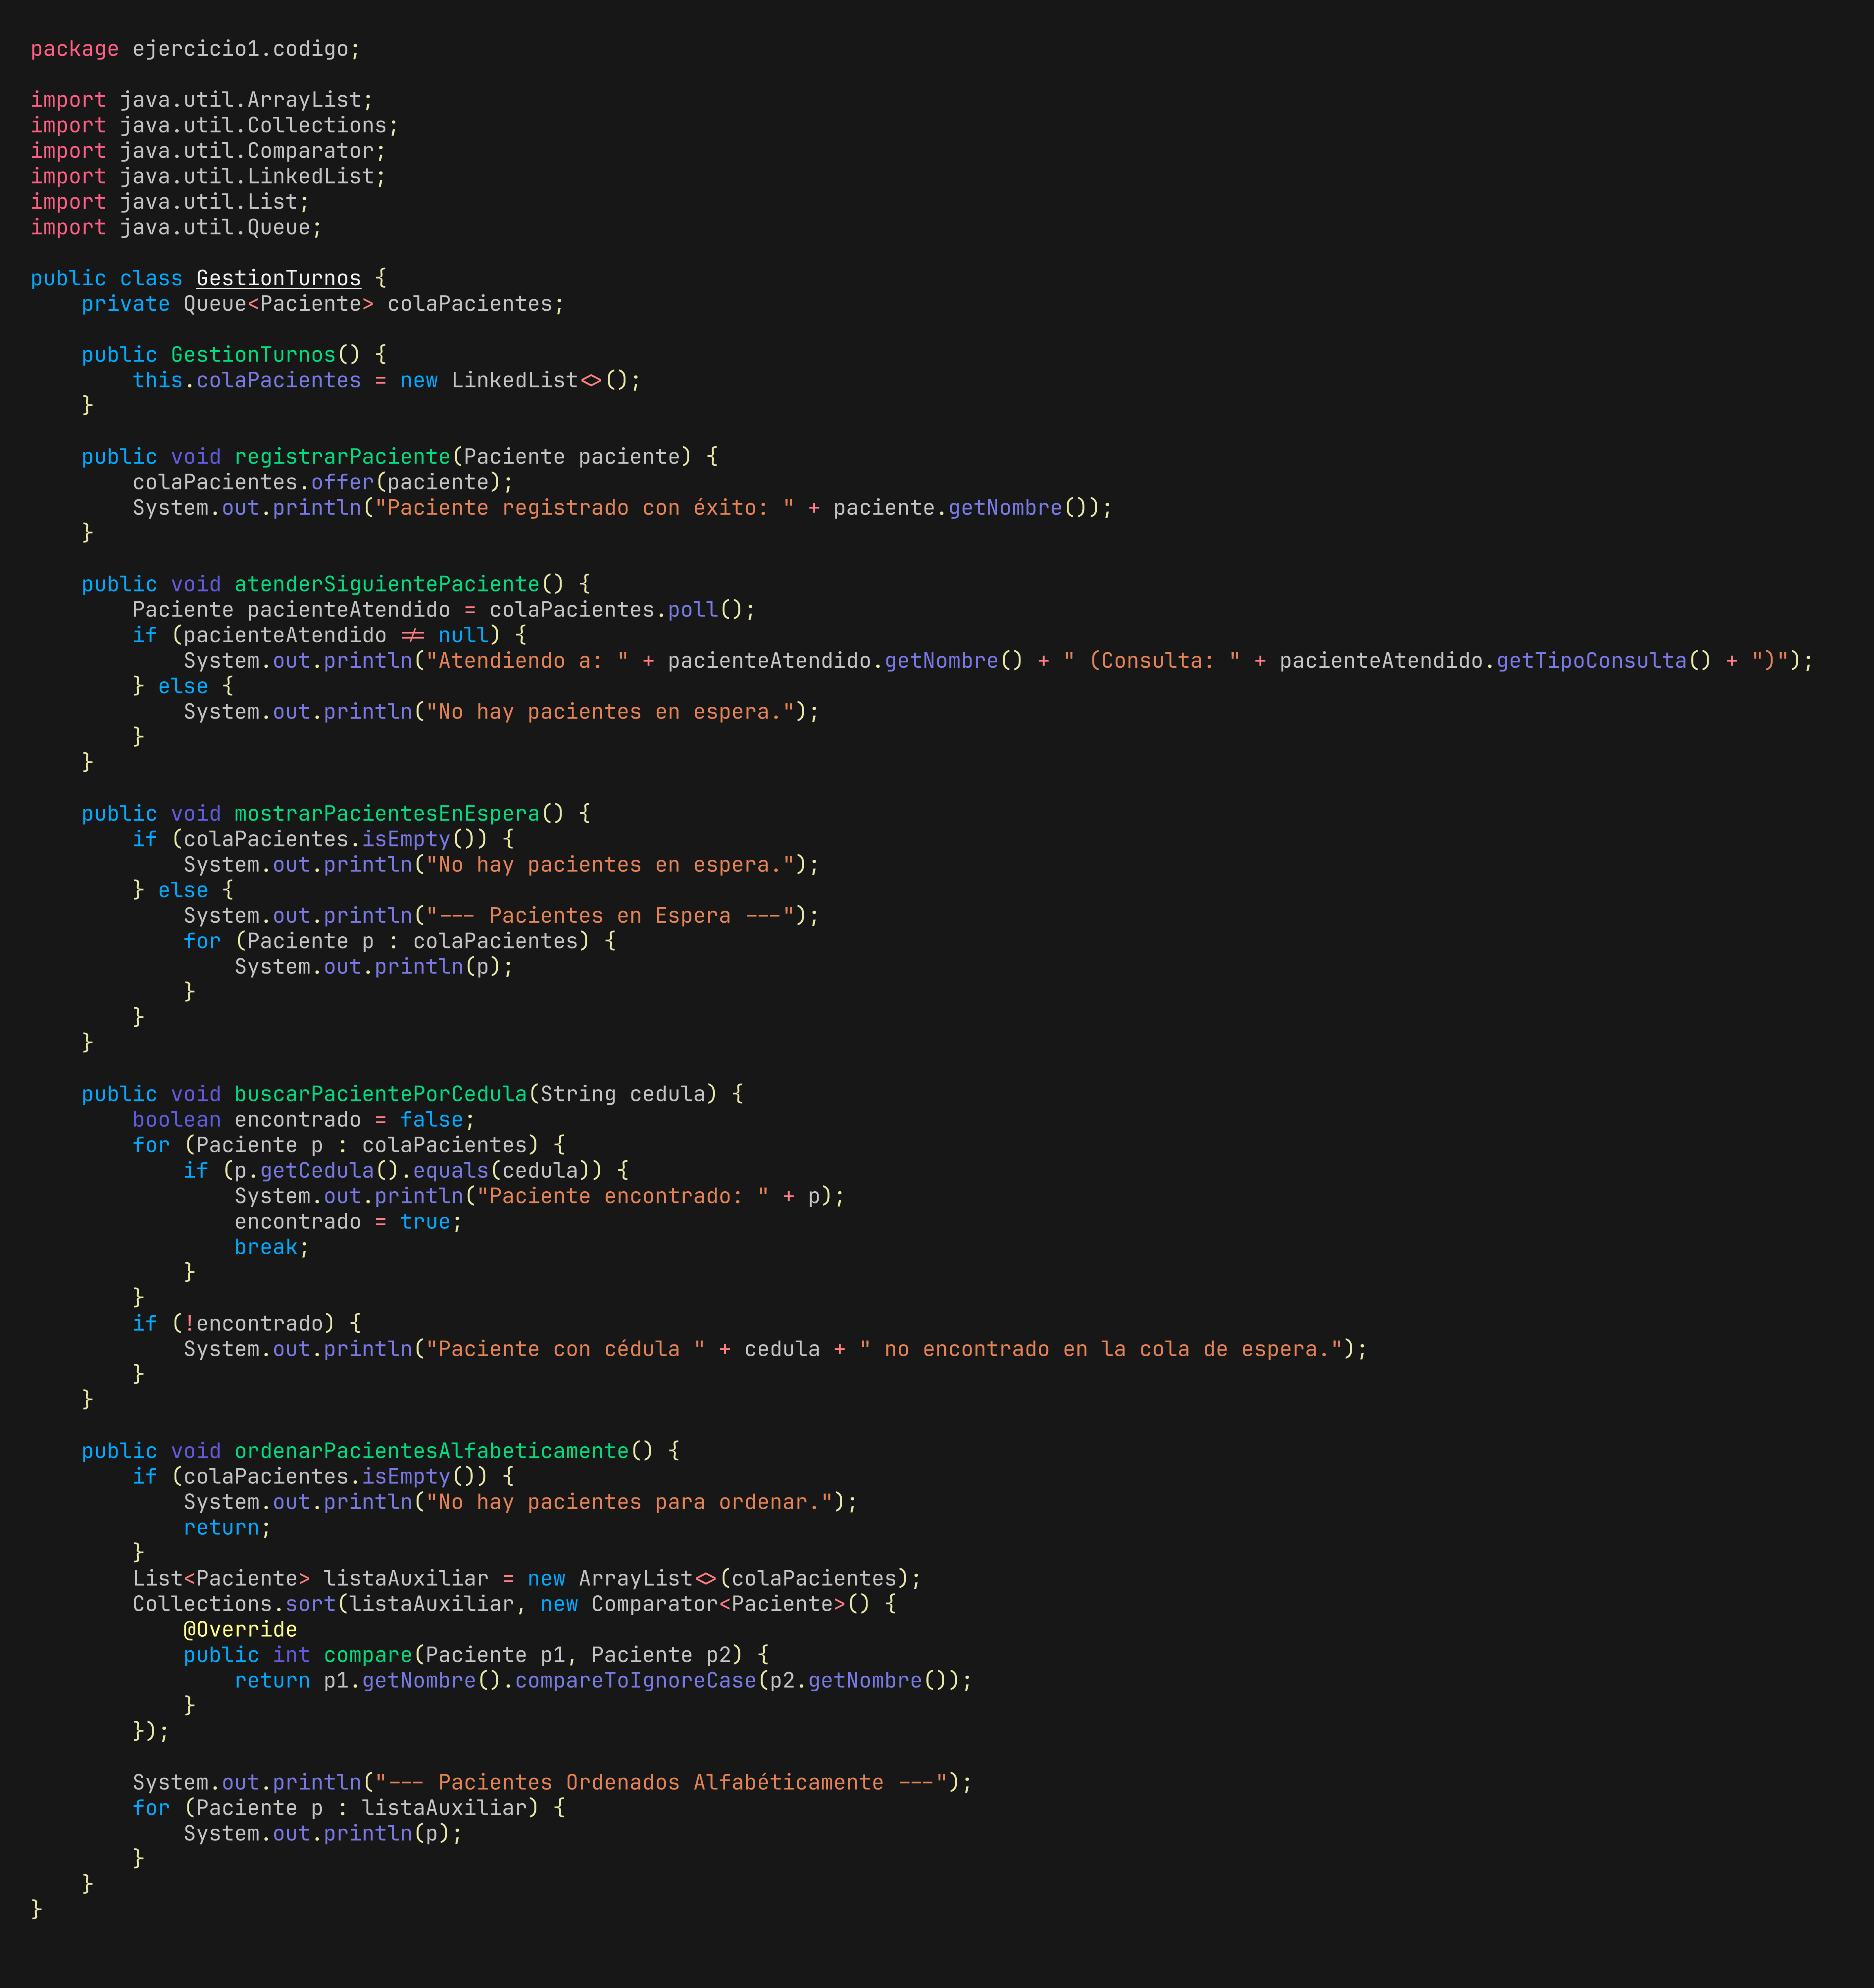
\includegraphics[width=0.8\textwidth]{ejercicio1/CAPTURAS_CODIGO/GestionTurnos.png}
    \caption{Código Fuente: GestionTurnos.png}
\end{figure}

\begin{figure}[H]
    \centering
    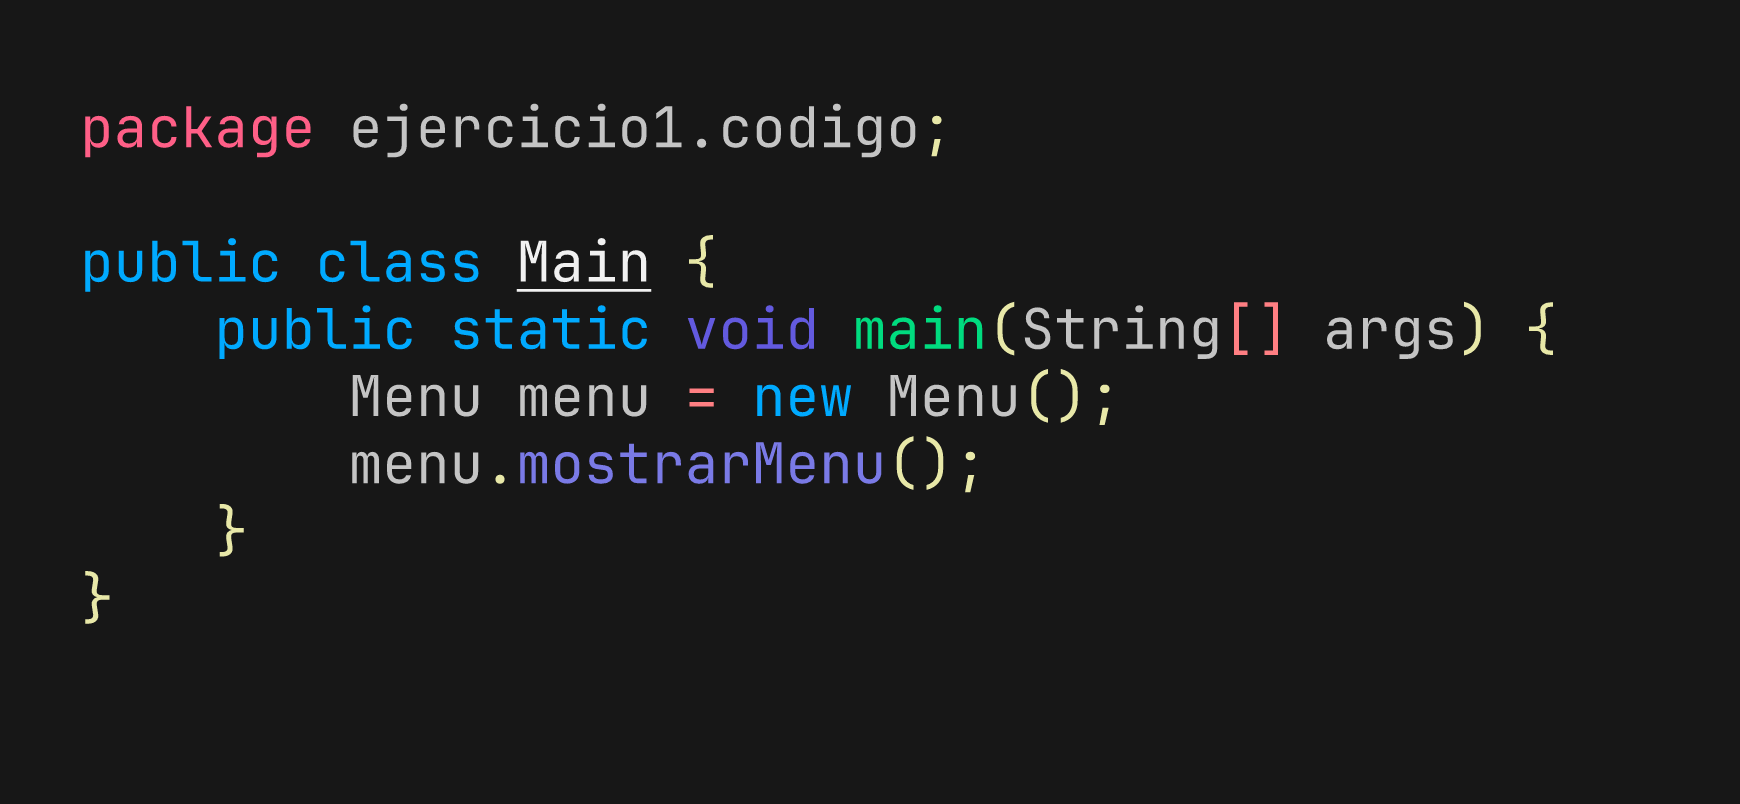
\includegraphics[width=0.8\textwidth]{ejercicio1/CAPTURAS_CODIGO/Main.png}
    \caption{Código Fuente: Main.png}
\end{figure}

\begin{figure}[H]
    \centering
    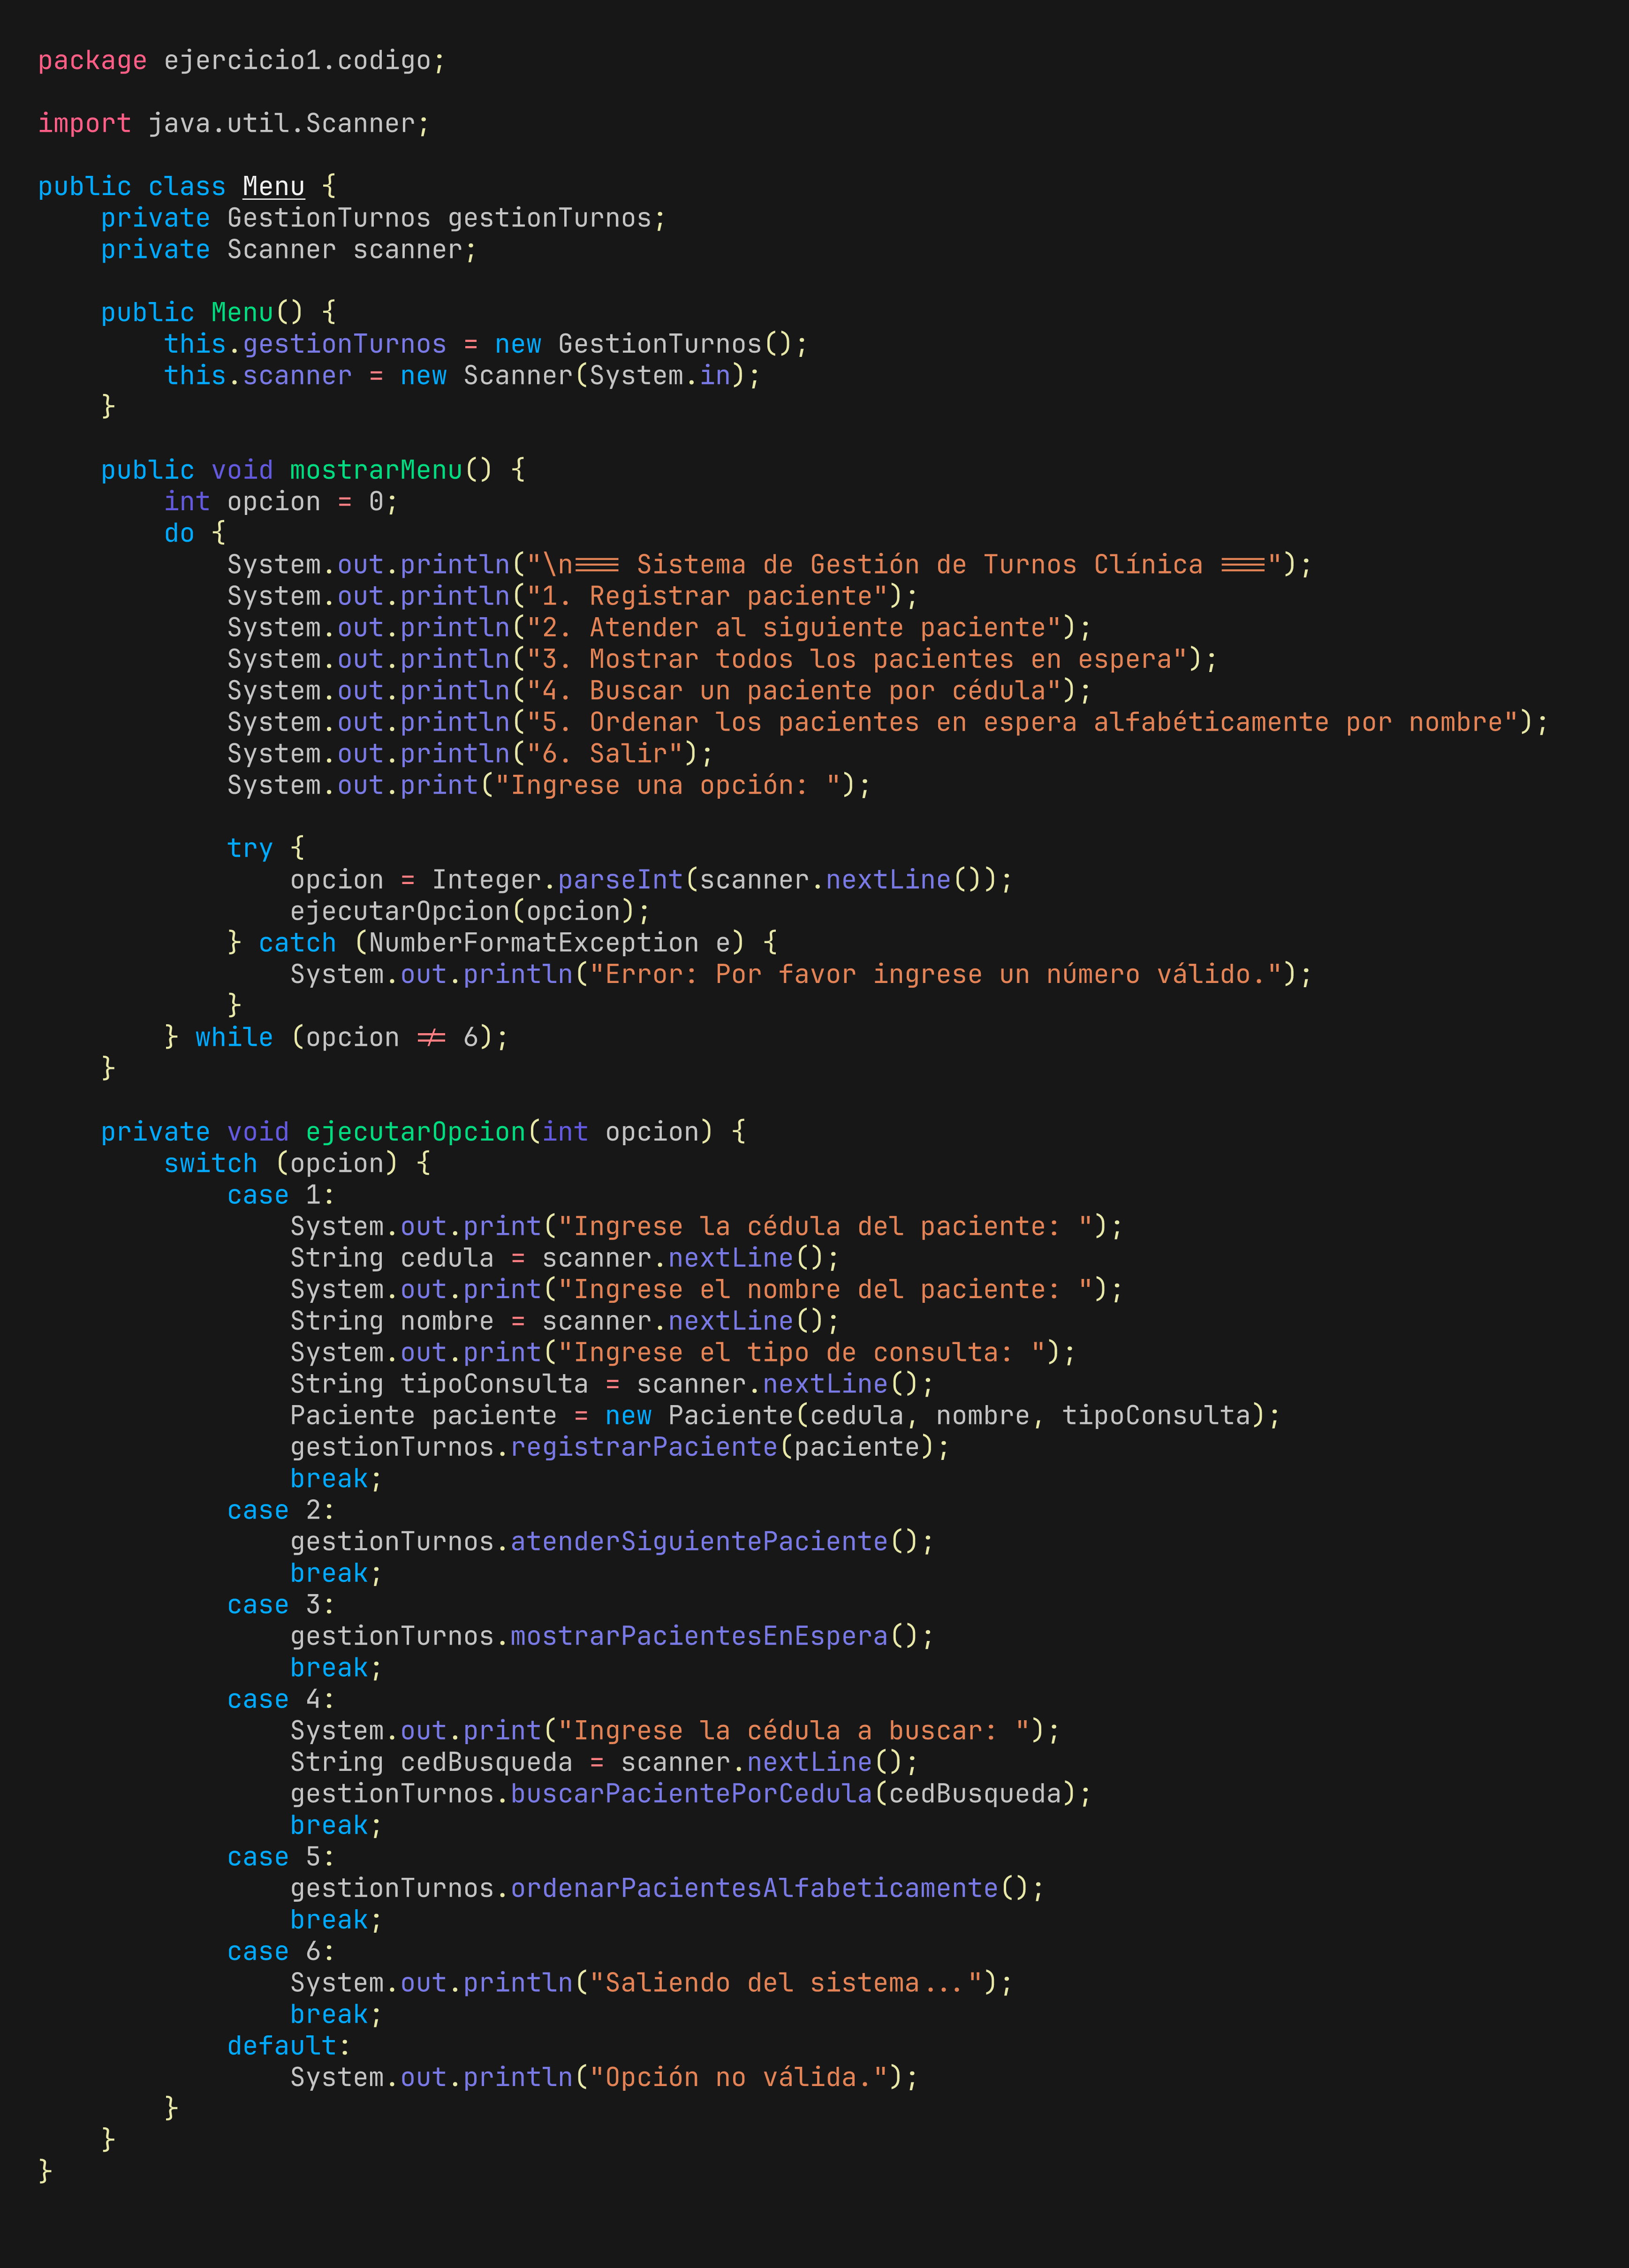
\includegraphics[width=0.8\textwidth]{ejercicio1/CAPTURAS_CODIGO/Menu.png}
    \caption{Código Fuente: Menu.png}
\end{figure}

\begin{figure}[H]
    \centering
    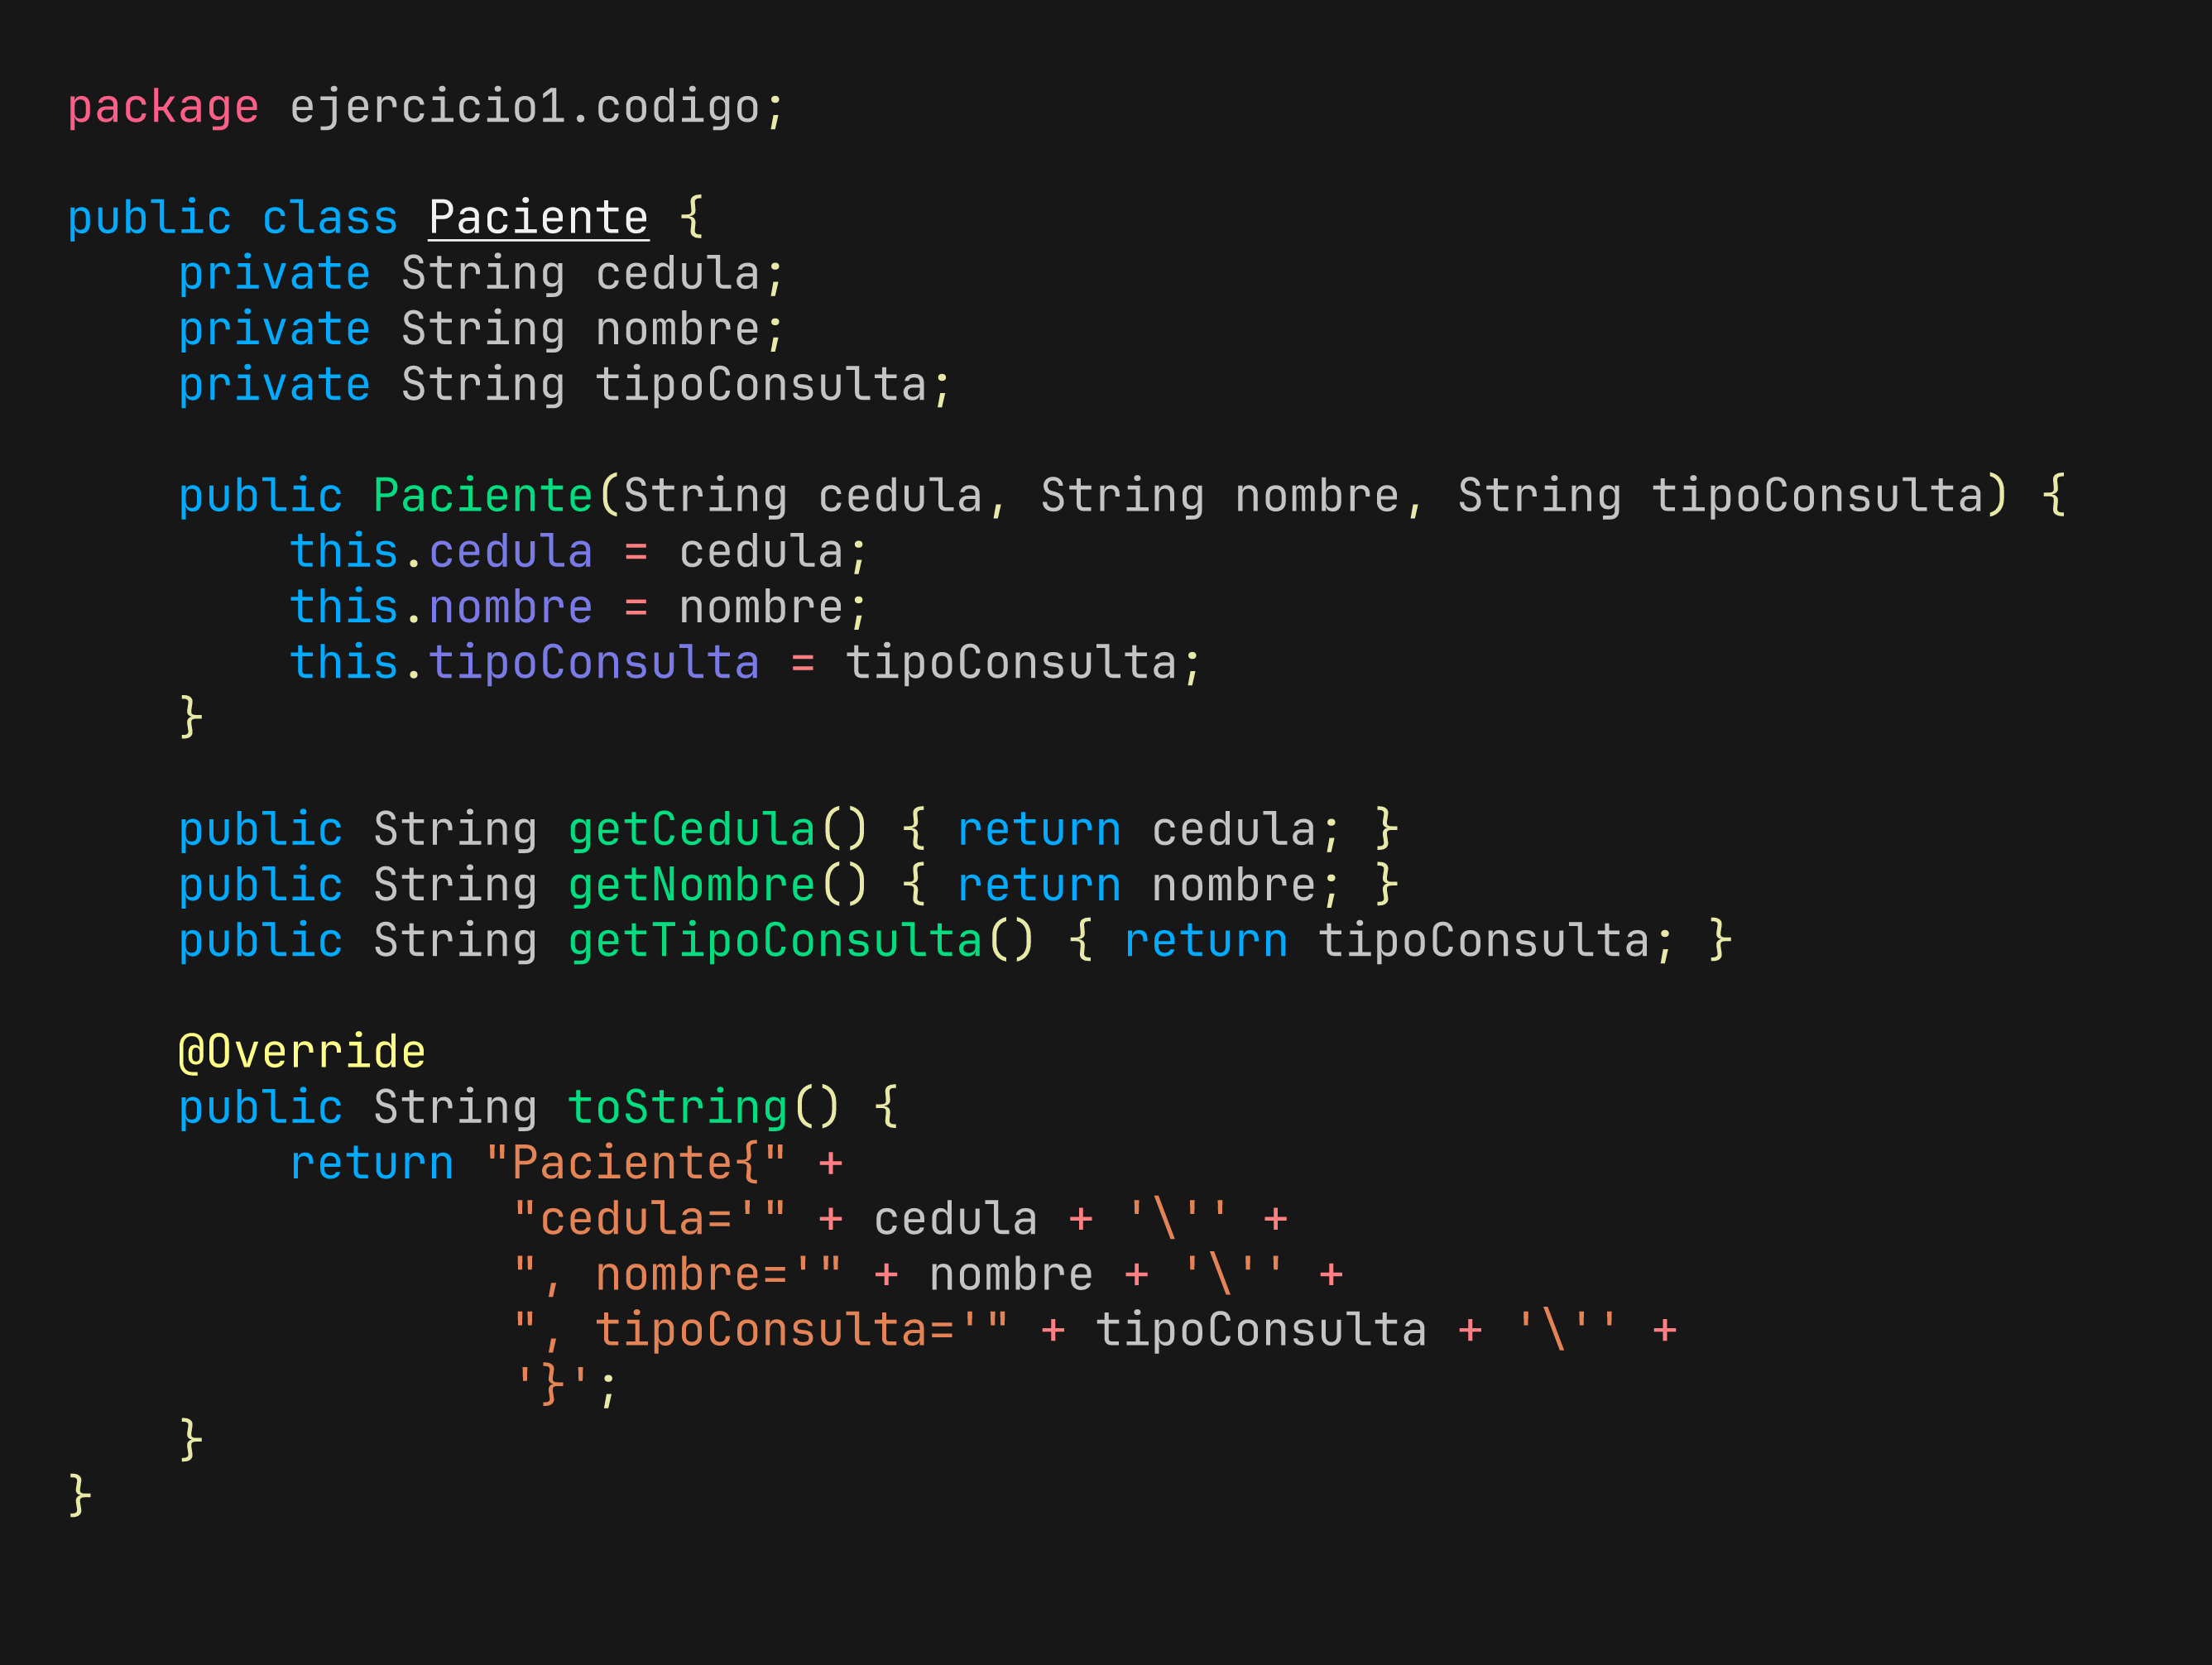
\includegraphics[width=0.8\textwidth]{ejercicio1/CAPTURAS_CODIGO/Paciente.png}
    \caption{Código Fuente: Paciente.png}
\end{figure}

\subsubsection*{Evidencias de Ejecución}
\begin{figure}[H]
    \centering
    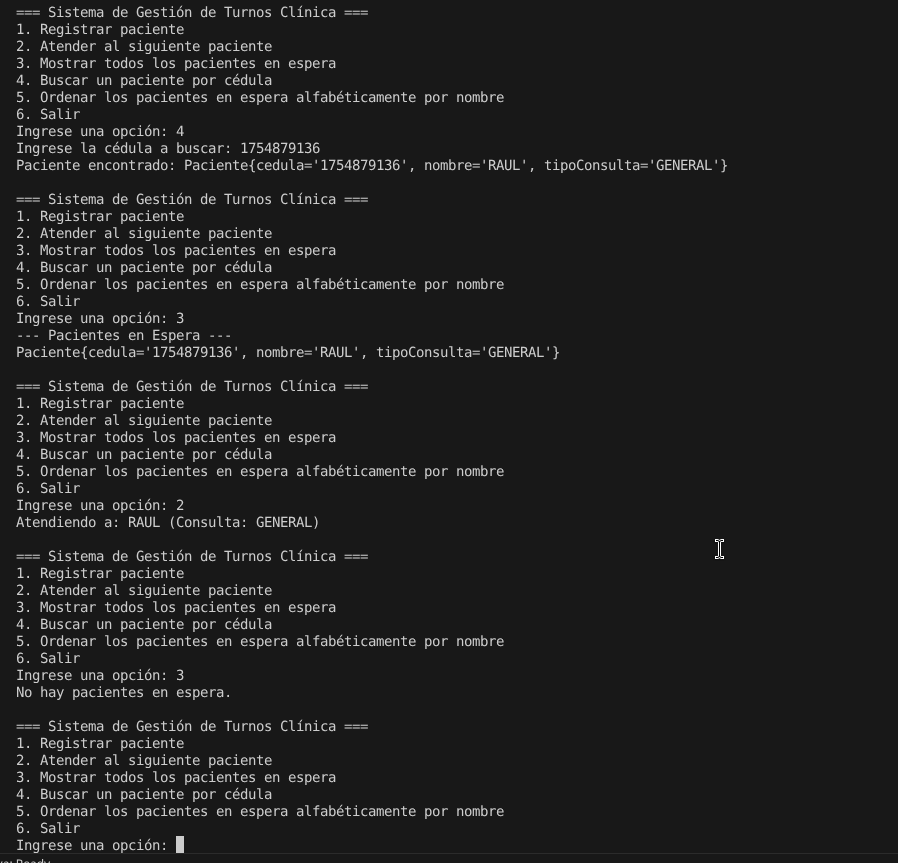
\includegraphics[width=0.8\textwidth]{ejercicio1/CAPTURAS_RESULTADO_CODIGO/image.png}
    \caption{Resultado de Ejecución - Reto 1}
\end{figure}

\subsection*{Reto 2}
Reto 2 - Caso de estudio: Historial de navegación usando pilas

Cree un programa que simule el historial de navegación de un navegador web. El estudiante debe implementar una pila donde se almacenen las páginas visitadas. El sistema debe permitir:
1. Visitar una nueva página
2. Volver a la página anterior
3. Mostrar el historial actual
4. Buscar si una página fue visitada
5. Ordenar alfabéticamente las páginas visitadas para mostrarlas como reporte

\subsubsection*{Capturas de Pantalla del Código}
\begin{figure}[H]
    \centering
    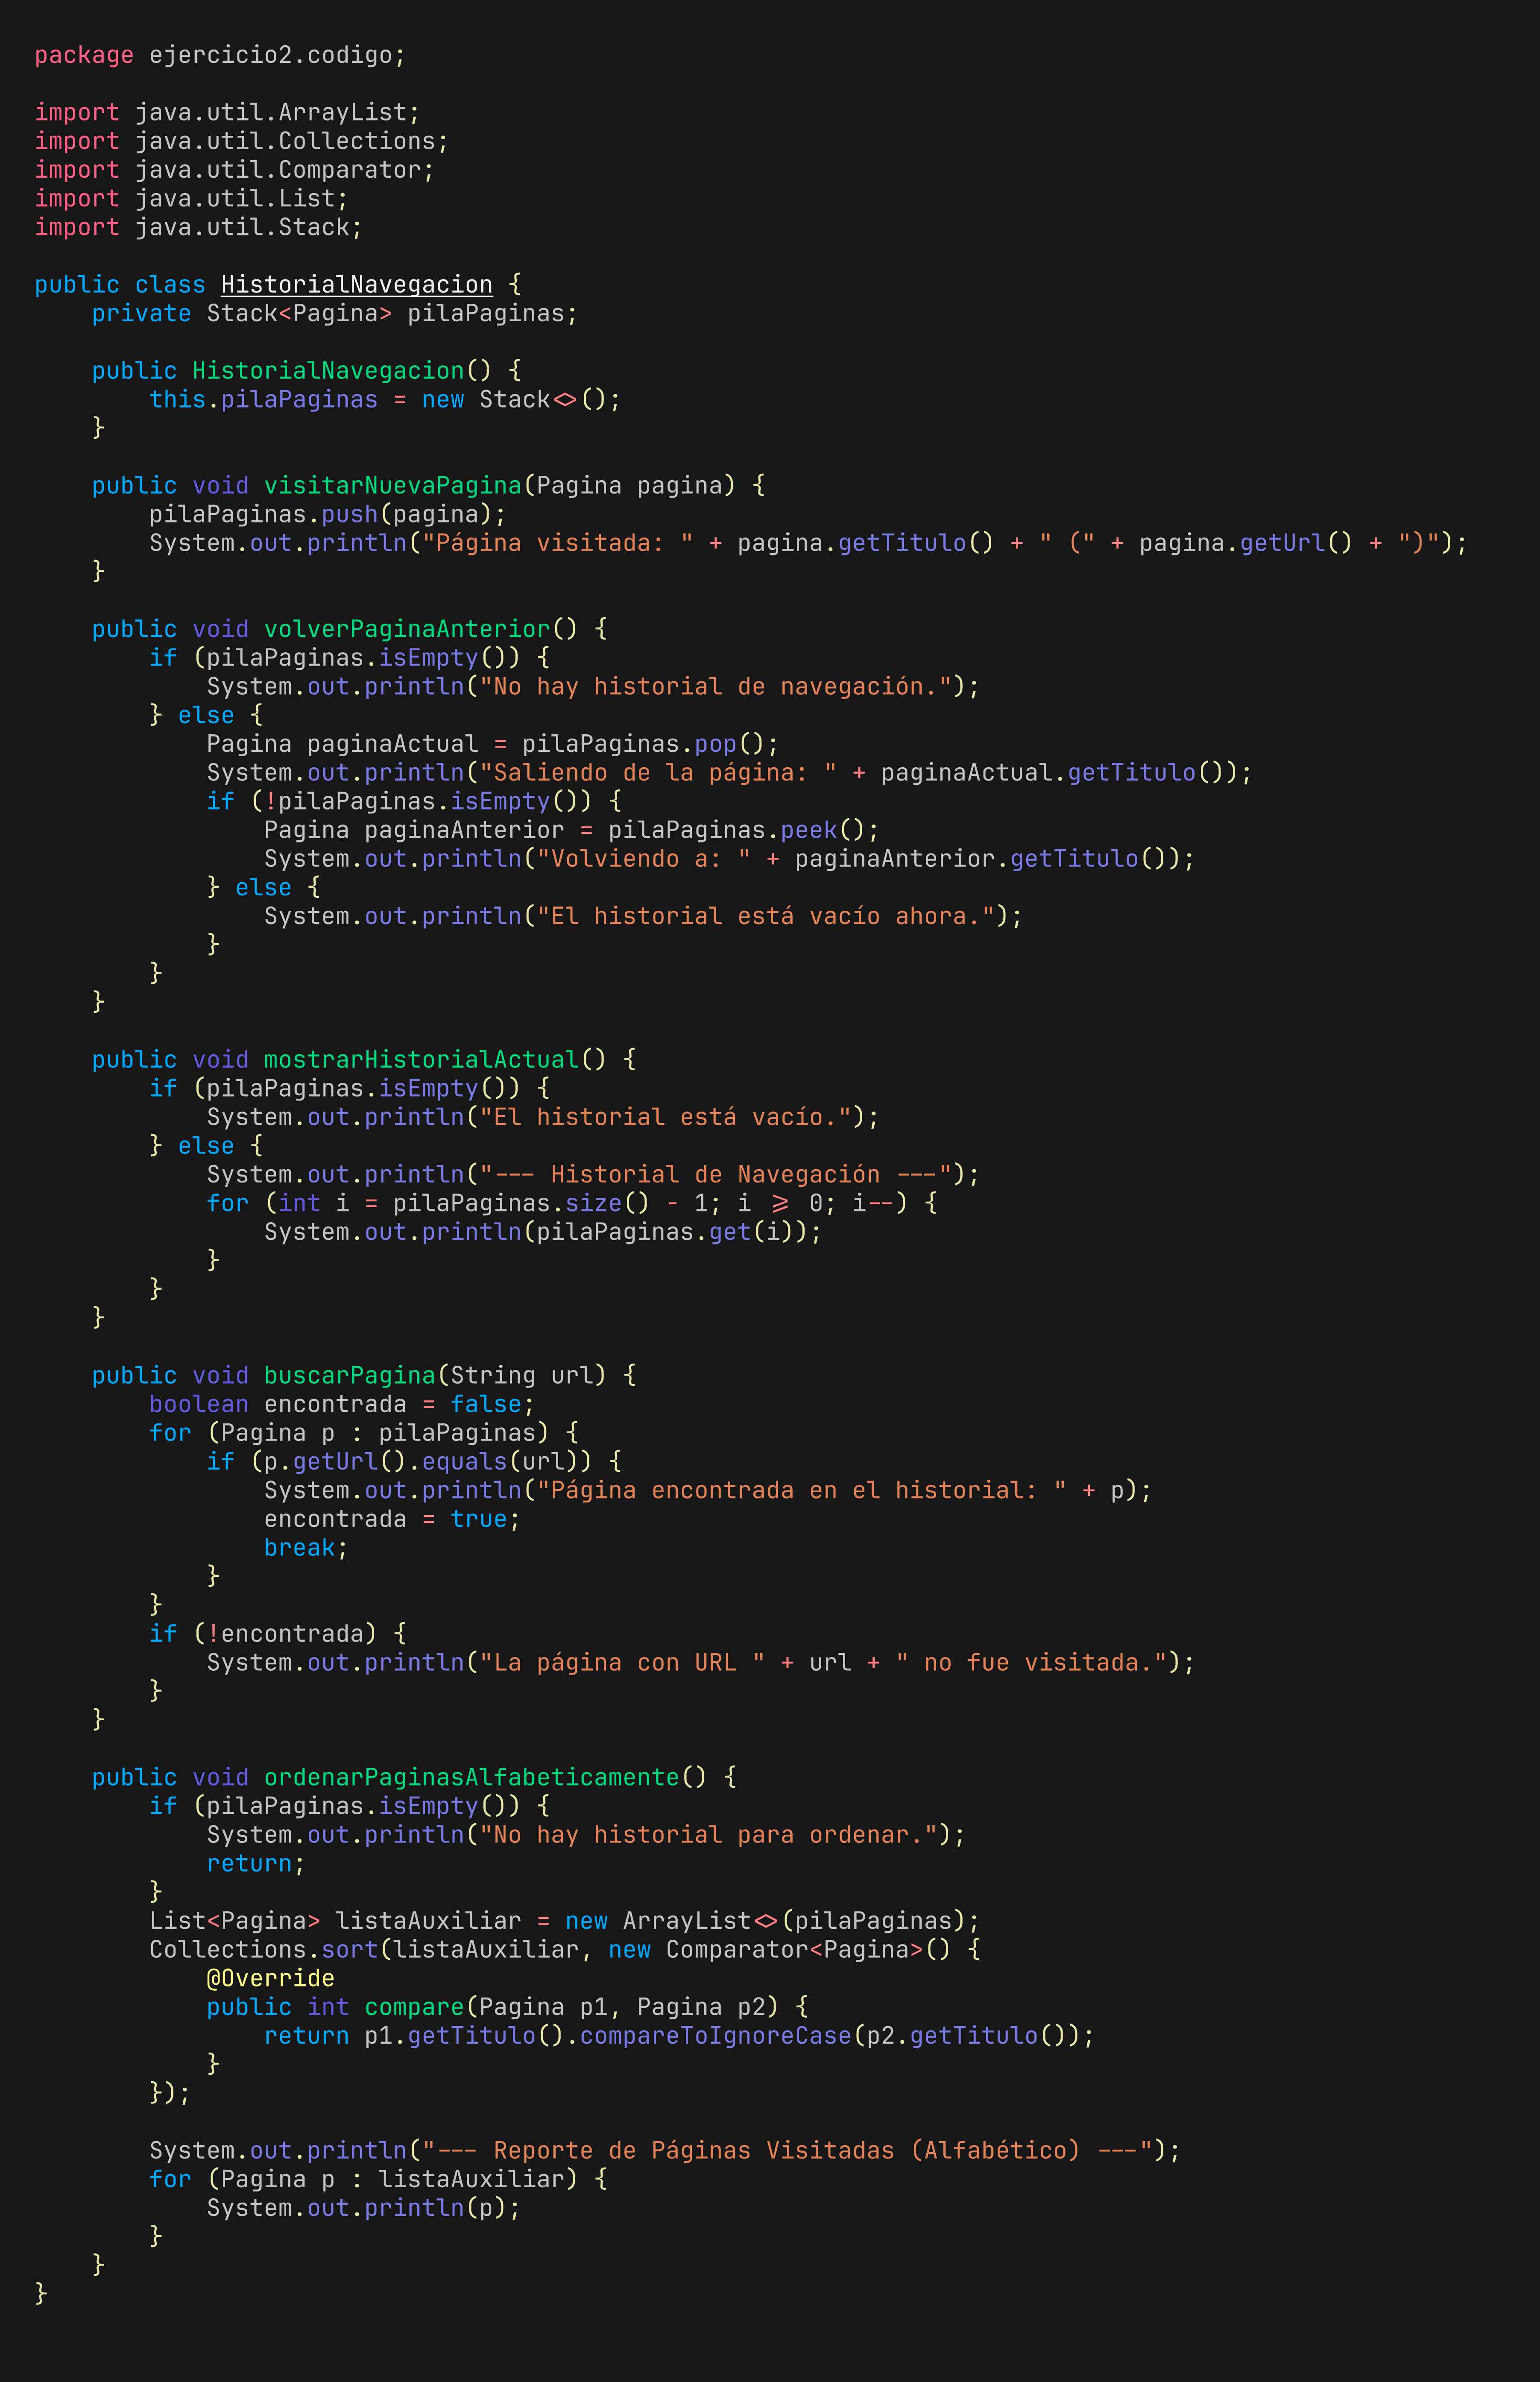
\includegraphics[width=0.8\textwidth]{ejercicio2/CAPTURAS_CODIGO/HistorialNavegacion.png}
    \caption{Código Fuente: HistorialNavegacion.png}
\end{figure}

\begin{figure}[H]
    \centering
    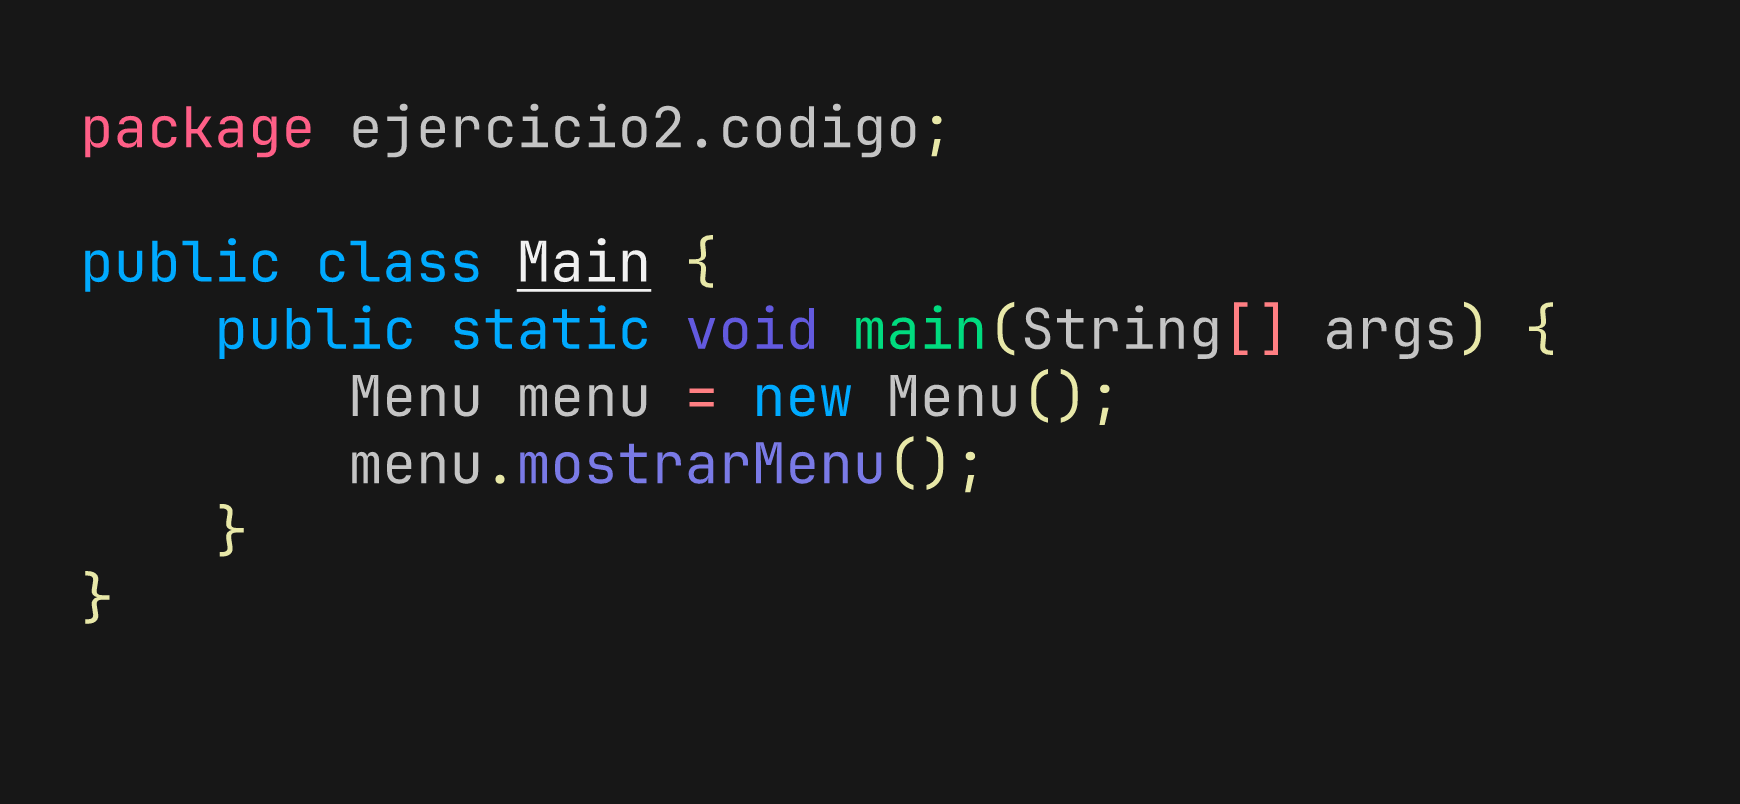
\includegraphics[width=0.8\textwidth]{ejercicio2/CAPTURAS_CODIGO/Main.png}
    \caption{Código Fuente: Main.png}
\end{figure}

\begin{figure}[H]
    \centering
    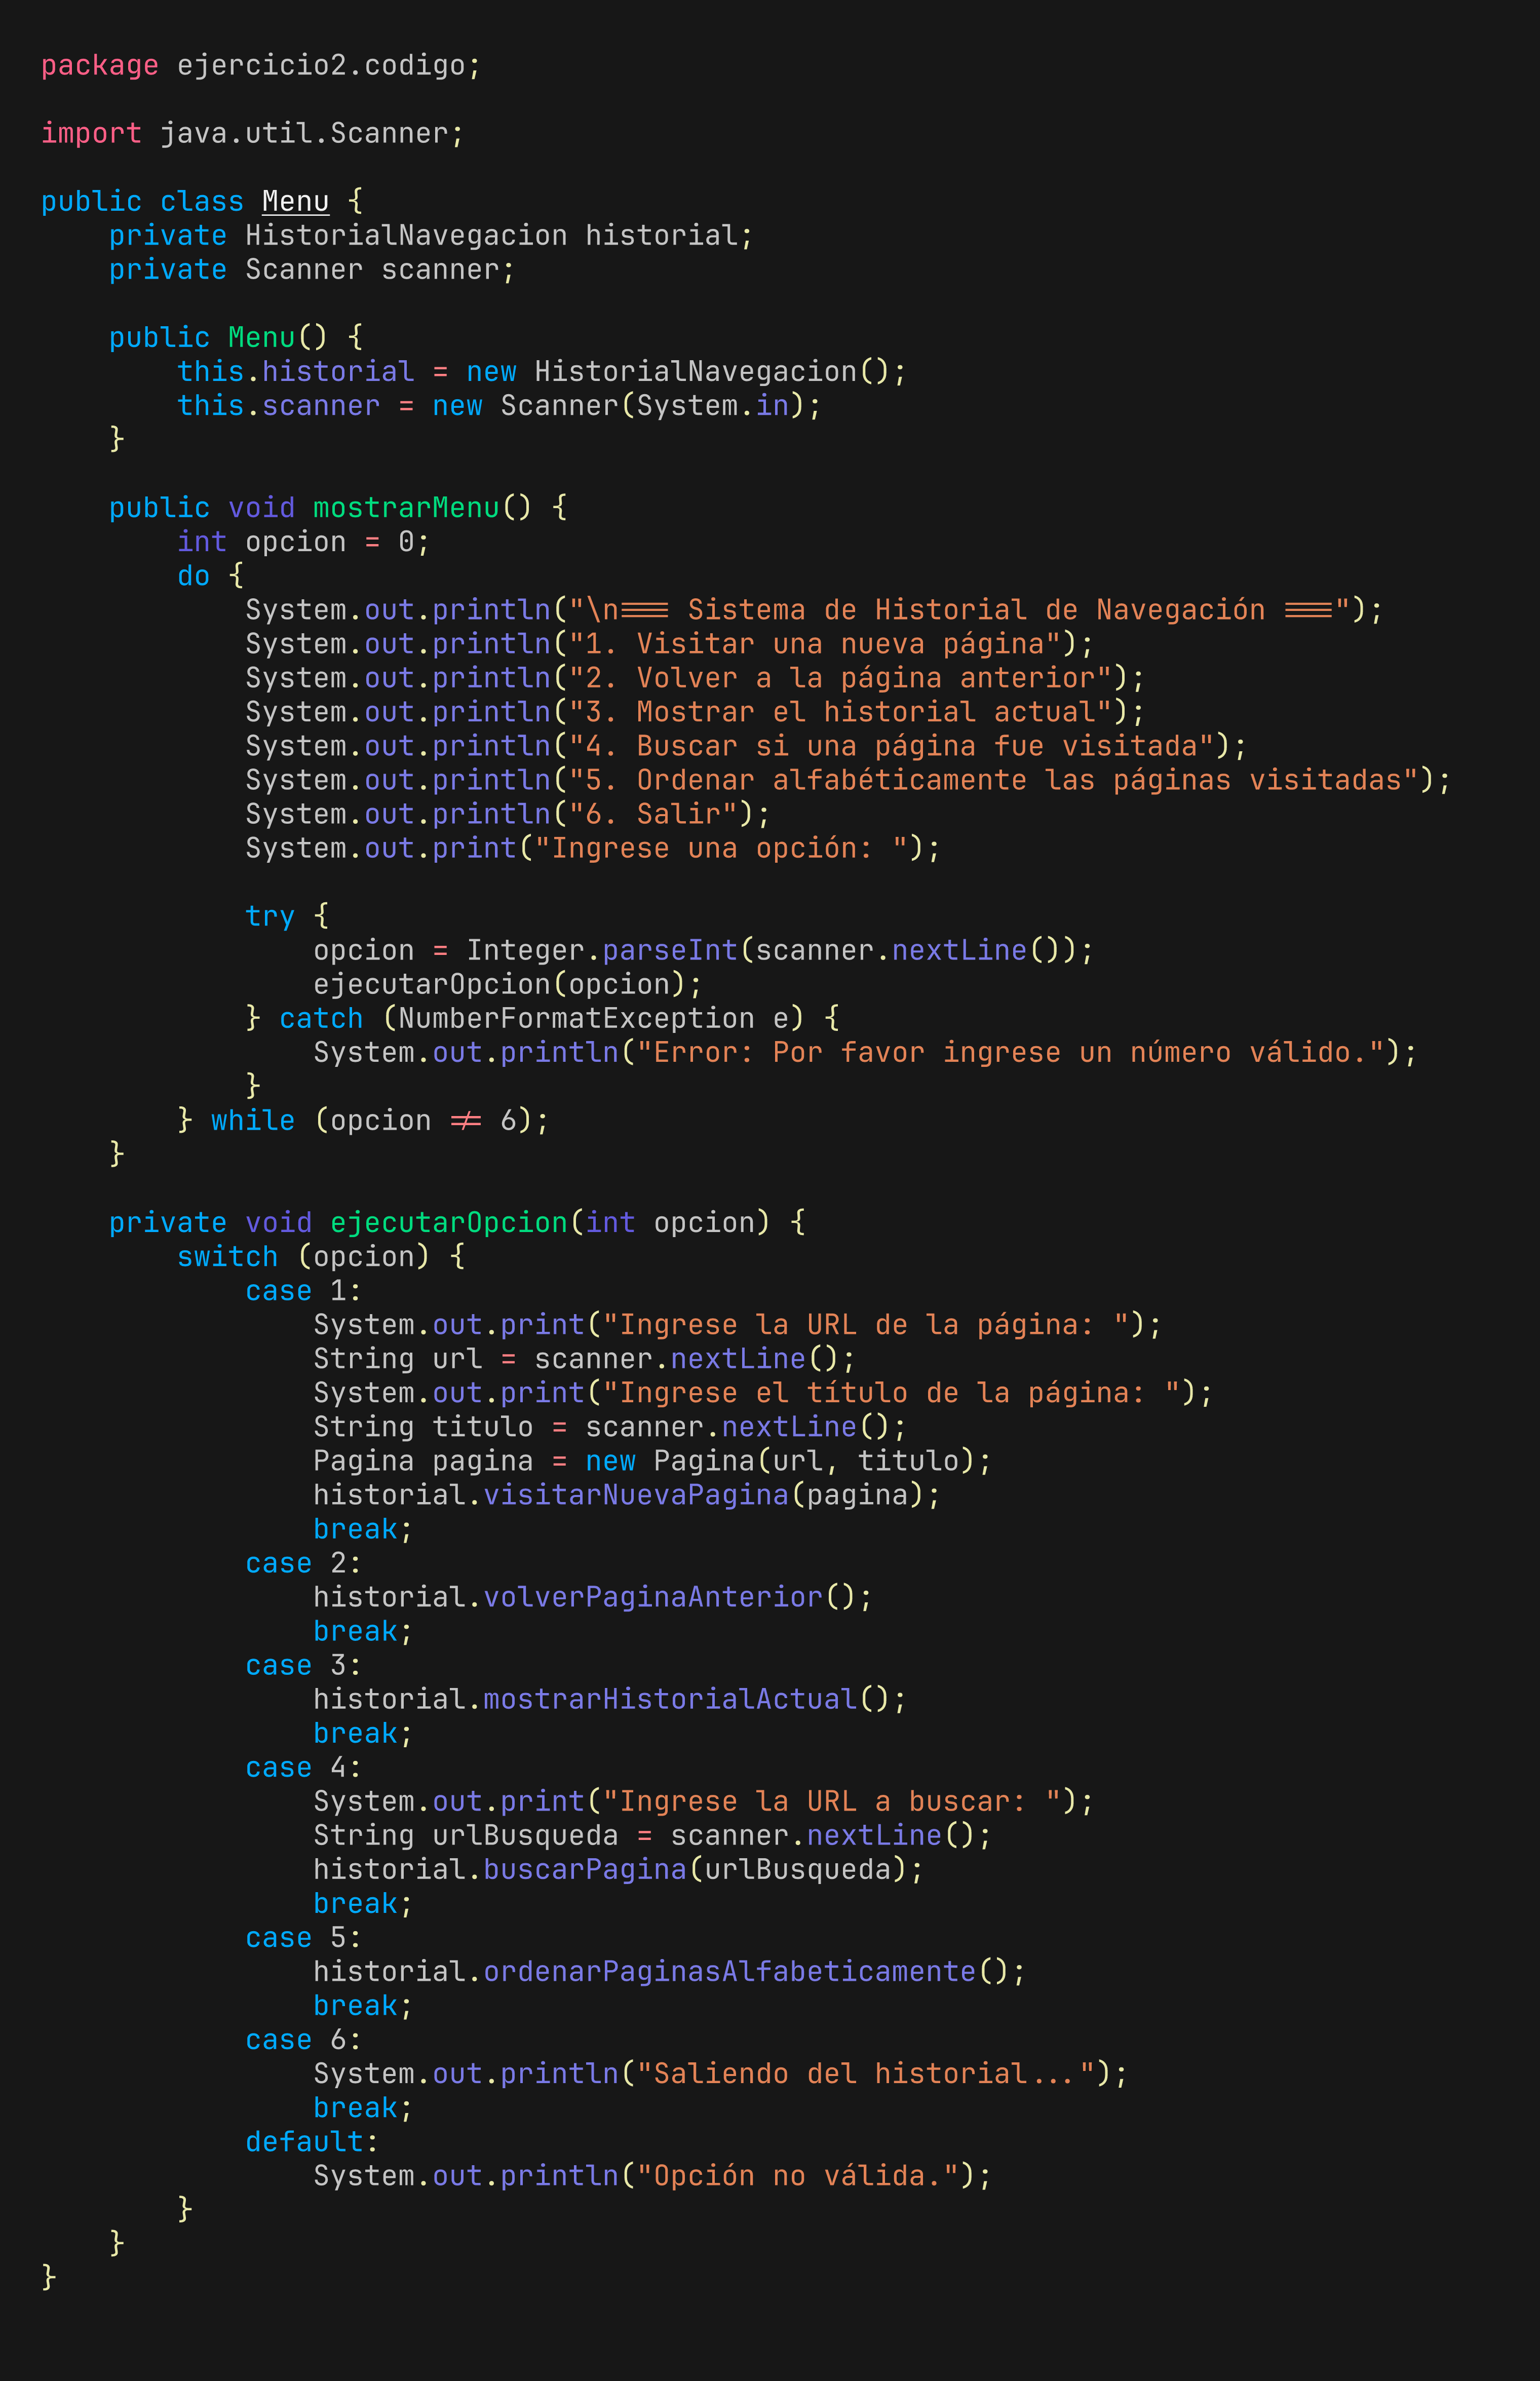
\includegraphics[width=0.8\textwidth]{ejercicio2/CAPTURAS_CODIGO/Menu.png}
    \caption{Código Fuente: Menu.png}
\end{figure}

\begin{figure}[H]
    \centering
    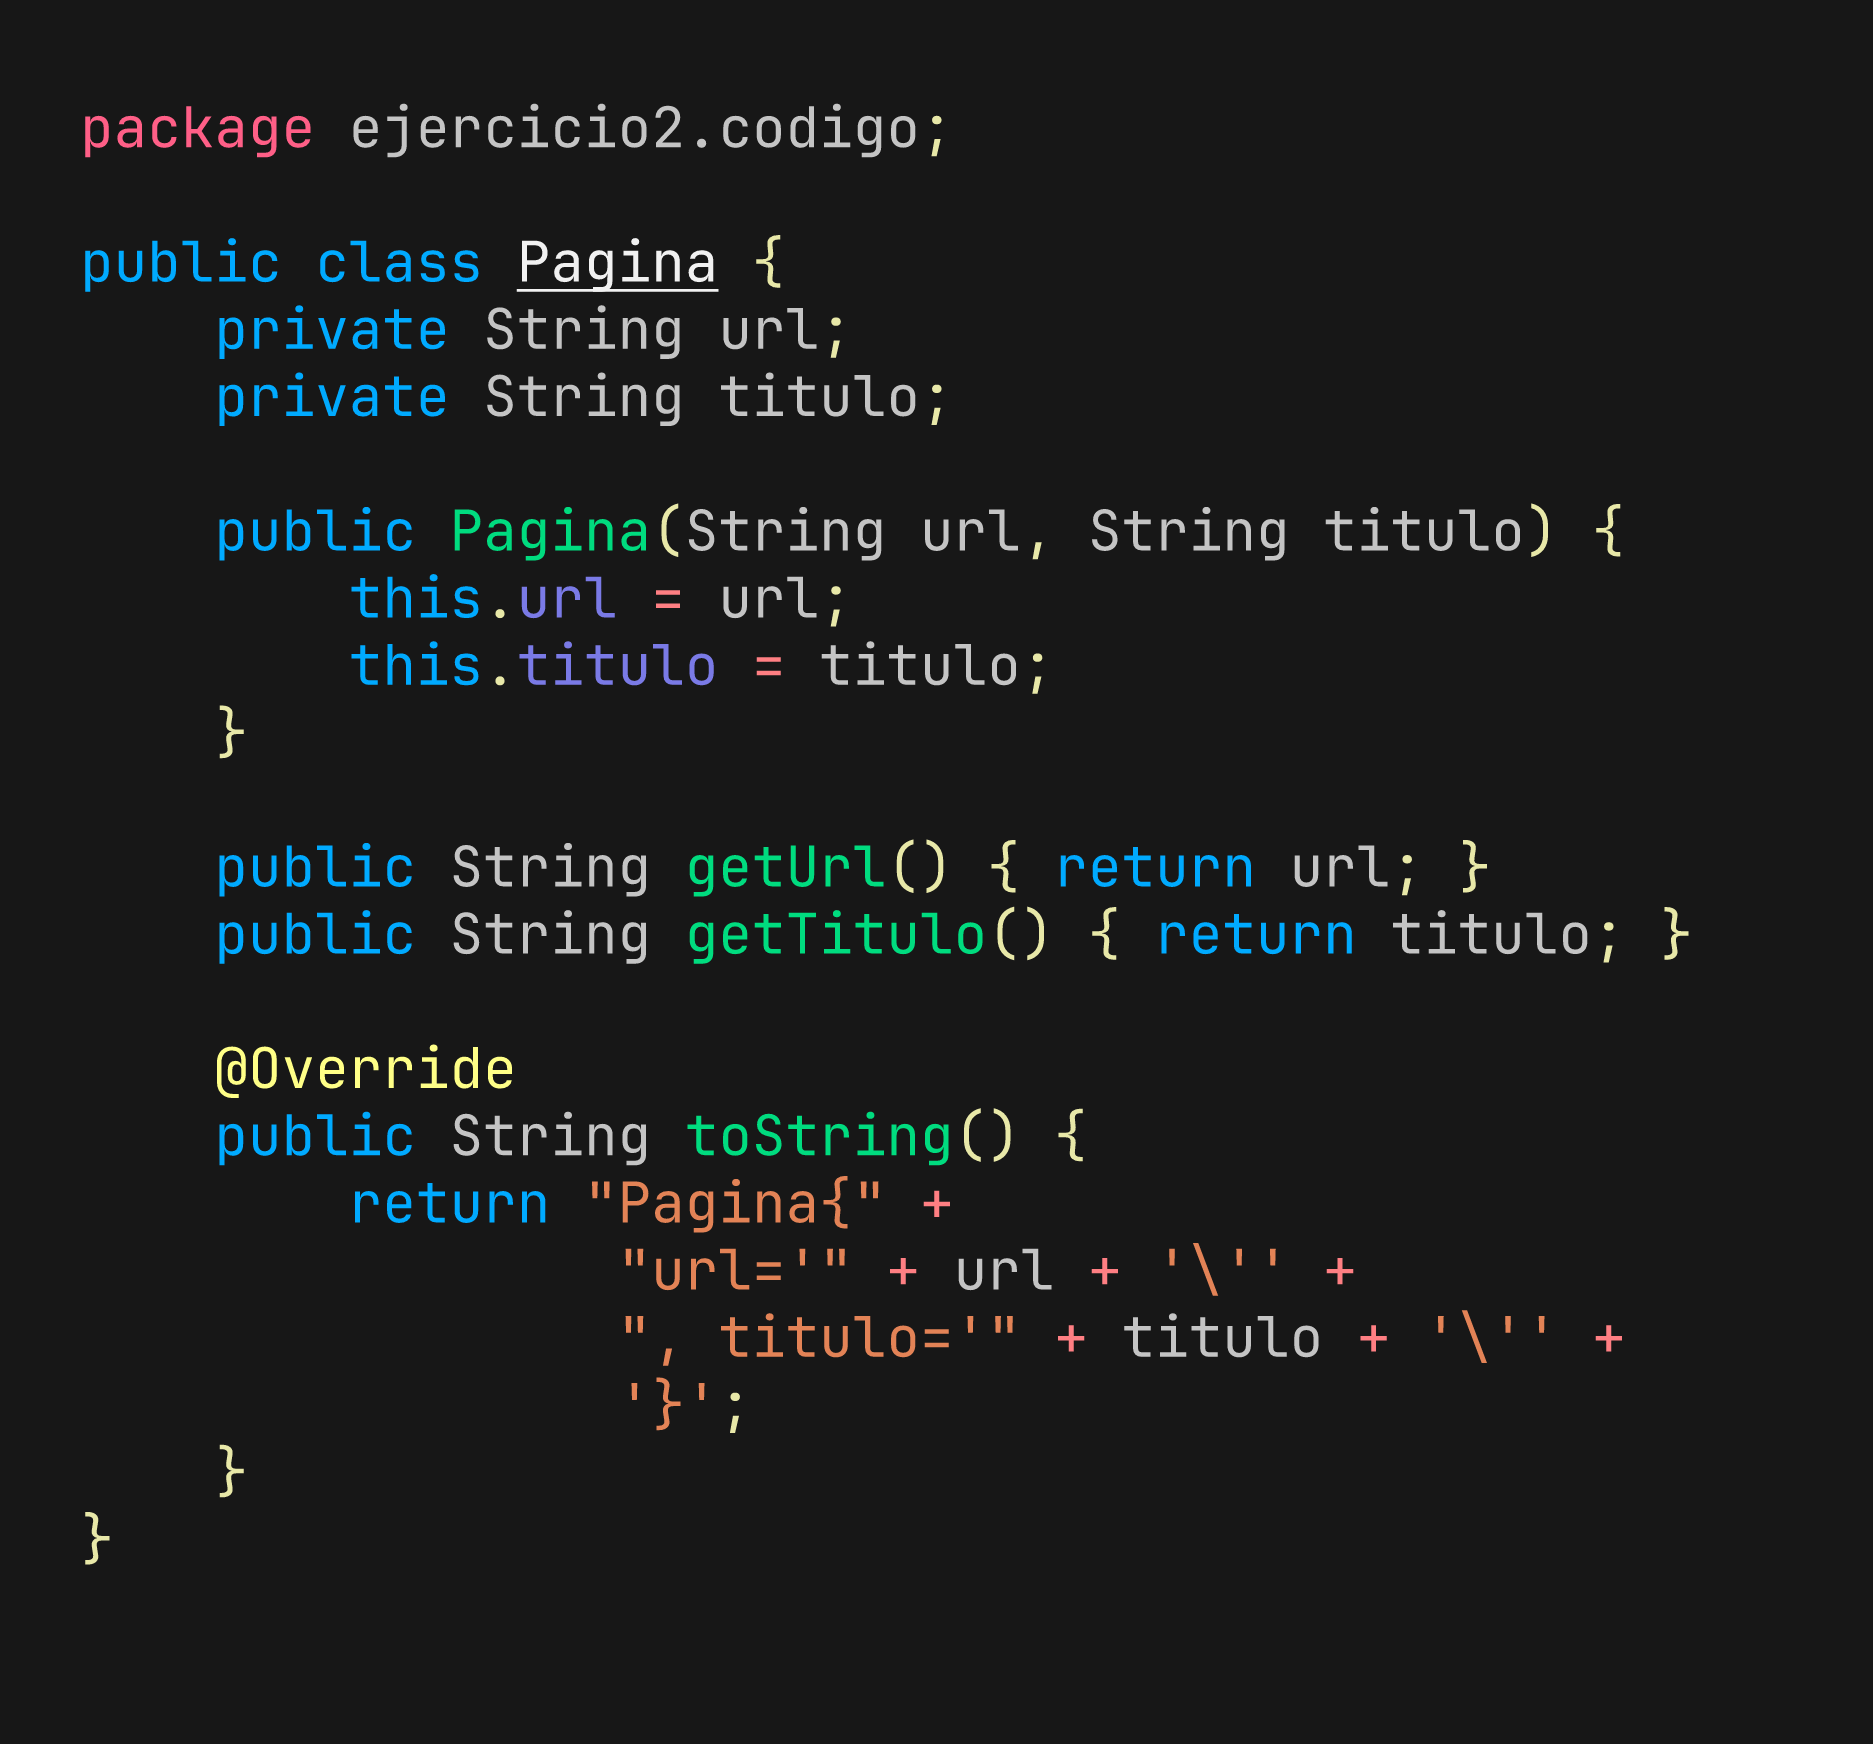
\includegraphics[width=0.8\textwidth]{ejercicio2/CAPTURAS_CODIGO/Pagina.png}
    \caption{Código Fuente: Pagina.png}
\end{figure}

\subsubsection*{Evidencias de Ejecución}
\begin{figure}[H]
    \centering
    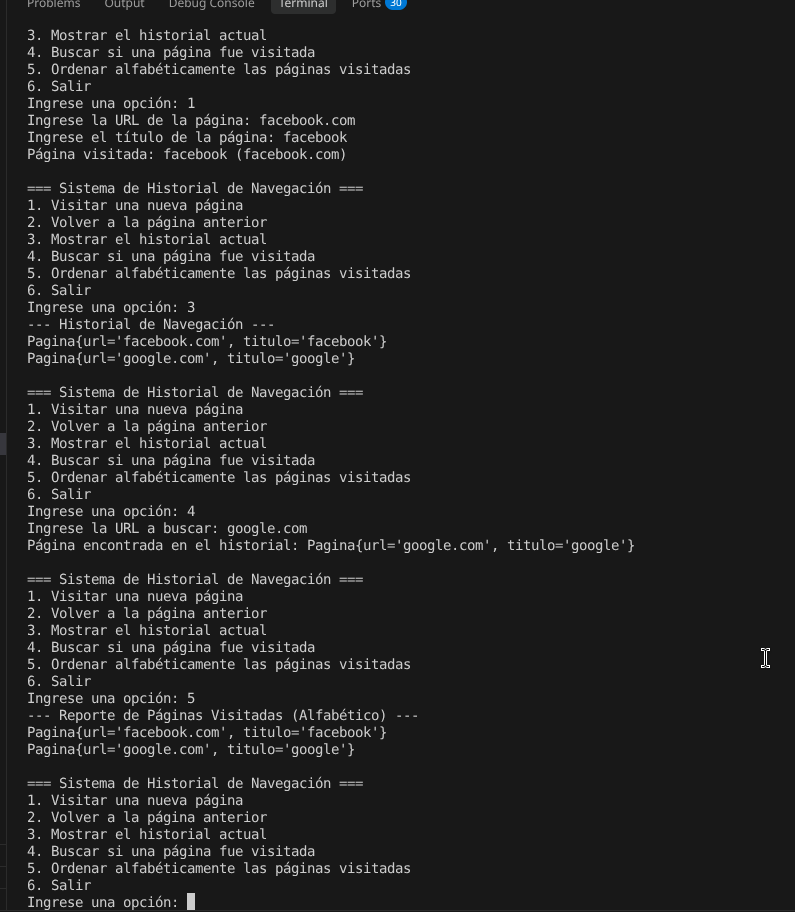
\includegraphics[width=0.8\textwidth]{ejercicio2/CAPTURAS_RESULTADO_CODIGO/image.png}
    \caption{Resultado de Ejecución - Reto 2}
\end{figure}

\subsection*{Reto 3}
Reto 3 - Caso de estudio: Registro de productos usando listas

Diseñe un programa para registrar productos de una tienda. Cada producto debe tener código, nombre, precio y stock. El sistema debe permitir:
1. Agregar productos
2. Listar todos los productos
3. Buscar un producto por código
4. Ordenar productos por precio de menor a mayor
5. Mostrar los productos con stock menor a 5 unidades

\subsubsection*{Capturas de Pantalla del Código}
\begin{figure}[H]
    \centering
    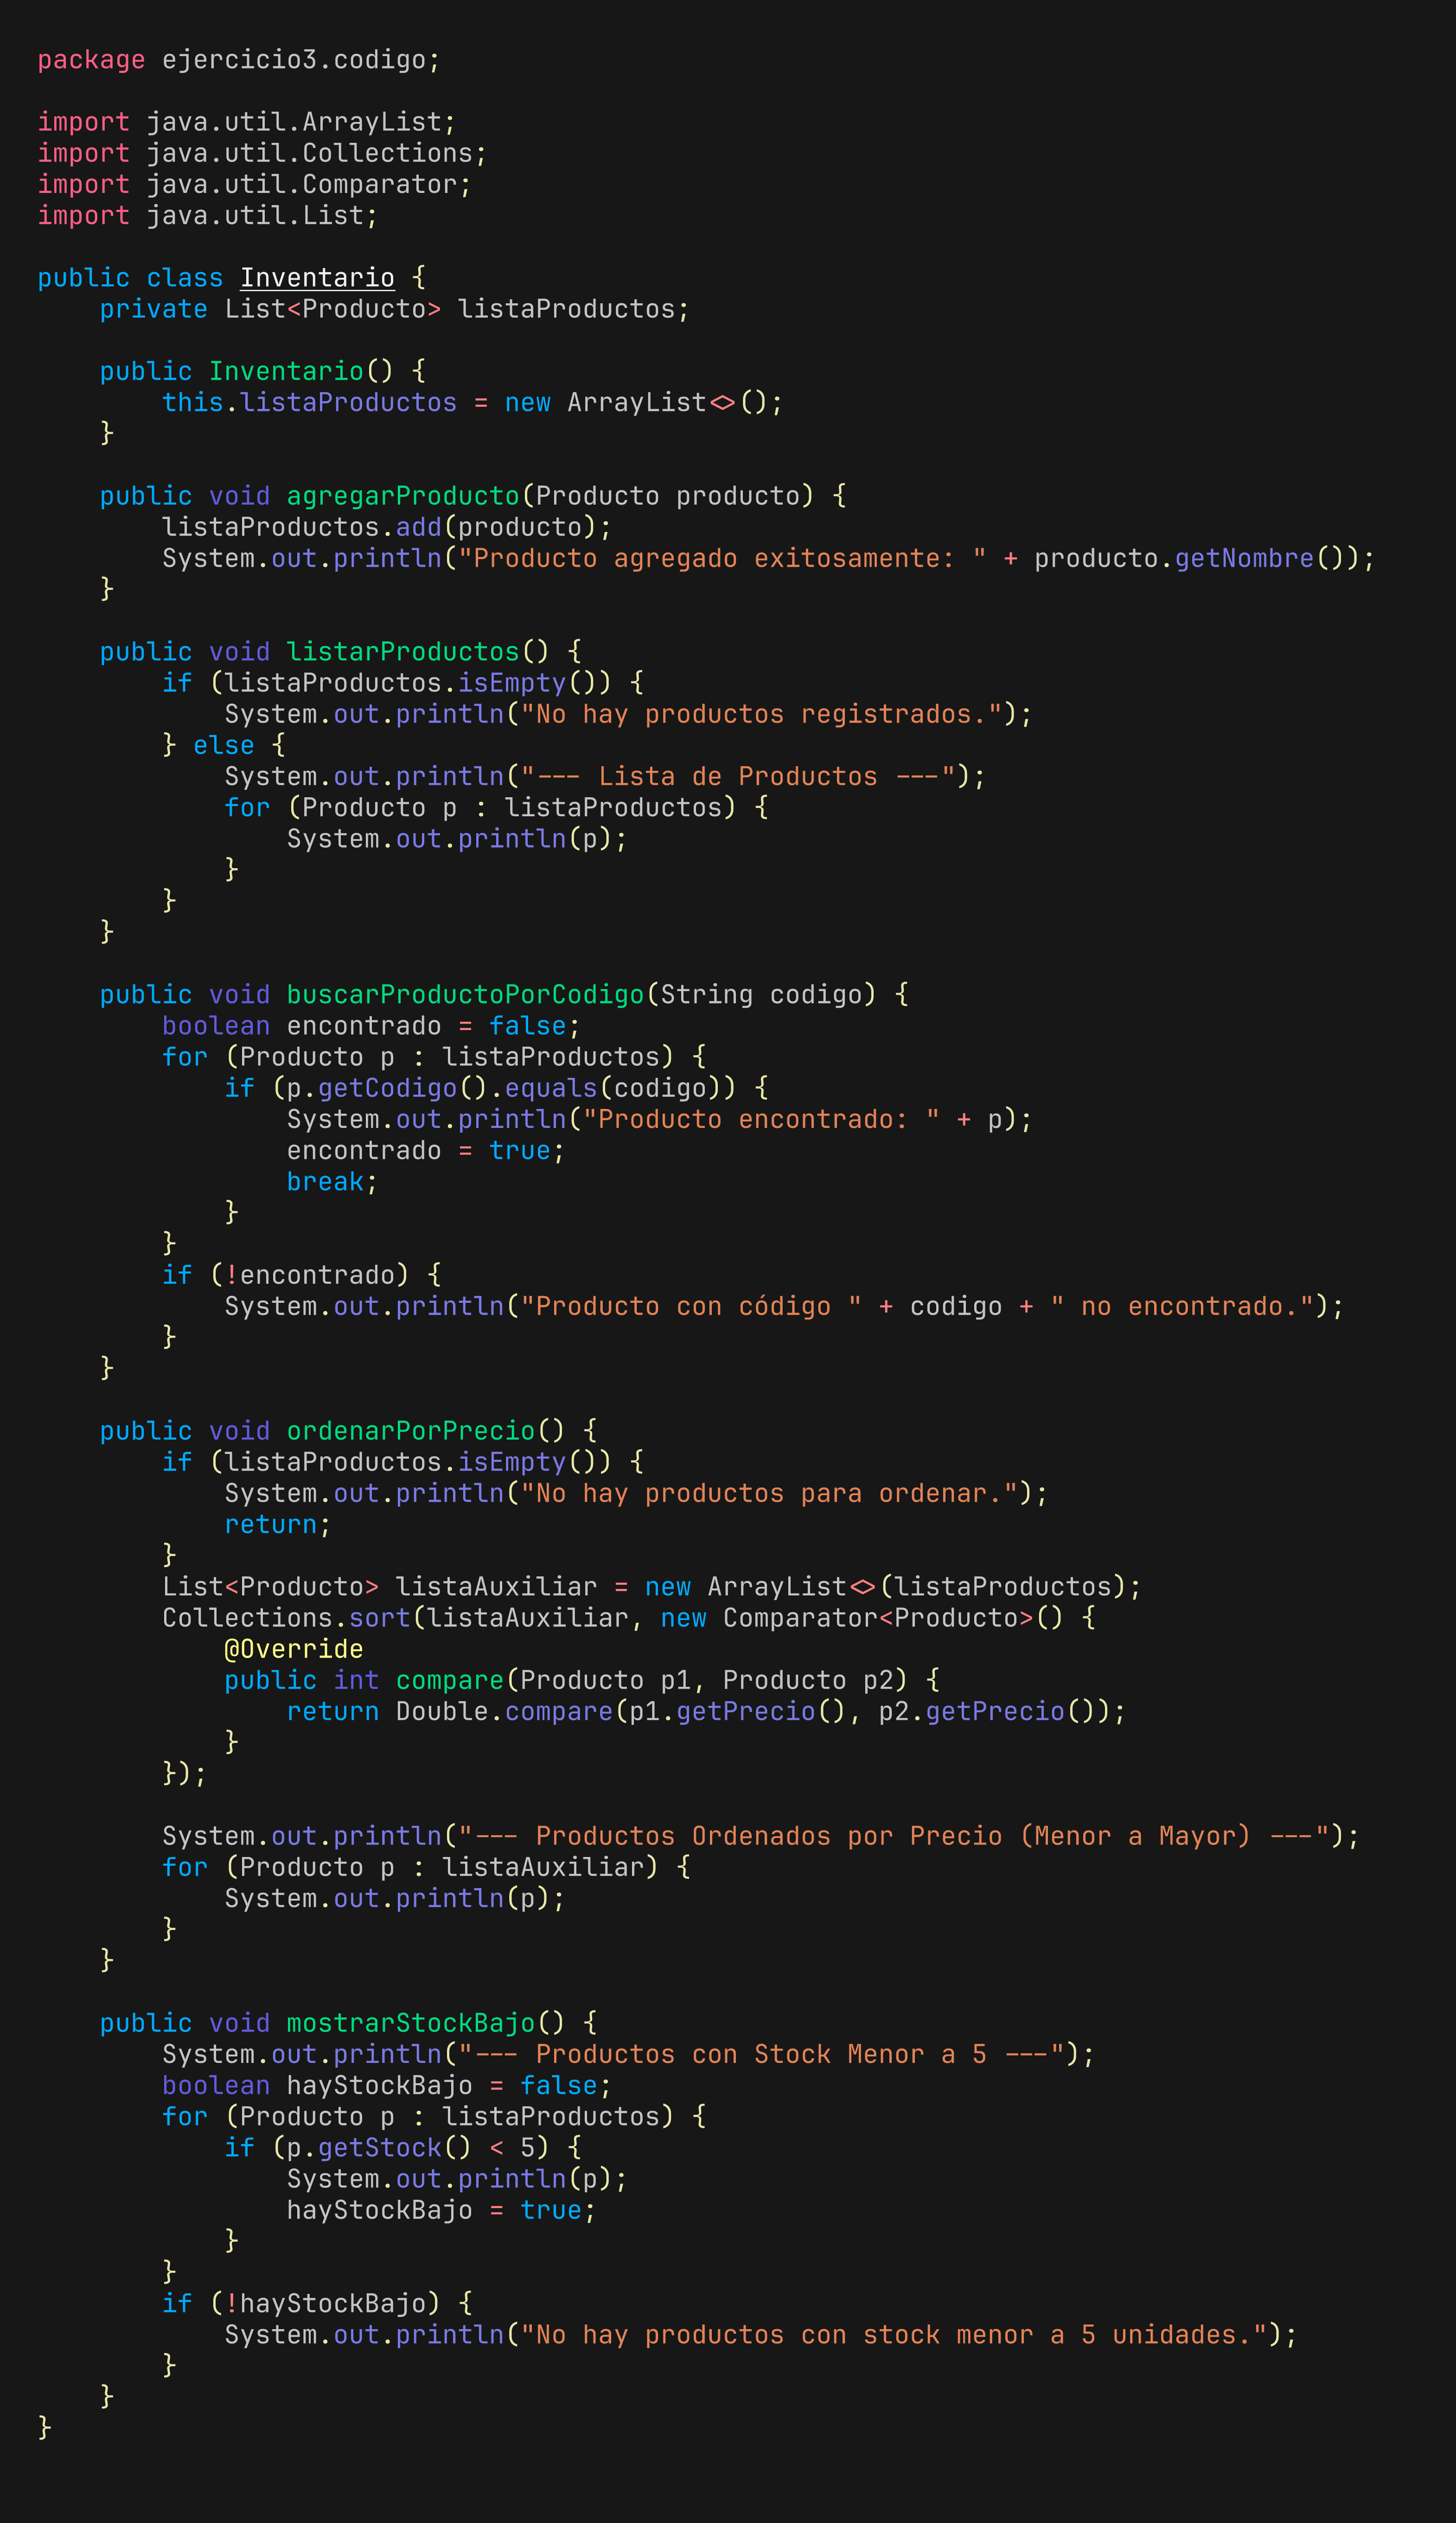
\includegraphics[width=0.8\textwidth]{ejercicio3/CAPTURAS_CODIGO/Inventario.png}
    \caption{Código Fuente: Inventario.png}
\end{figure}

\begin{figure}[H]
    \centering
    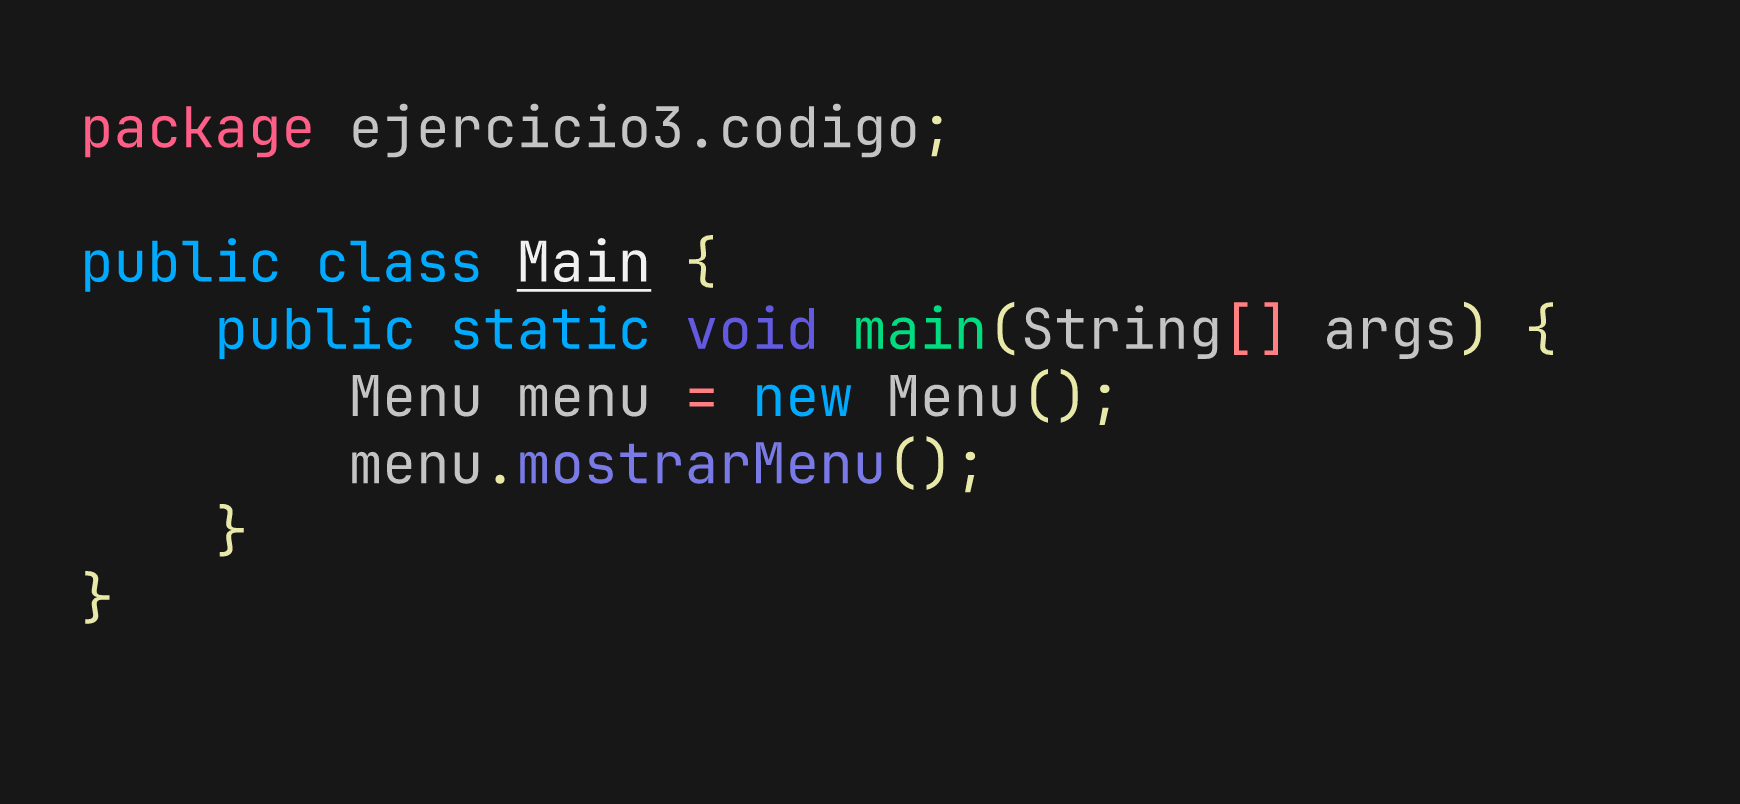
\includegraphics[width=0.8\textwidth]{ejercicio3/CAPTURAS_CODIGO/Main.png}
    \caption{Código Fuente: Main.png}
\end{figure}

\begin{figure}[H]
    \centering
    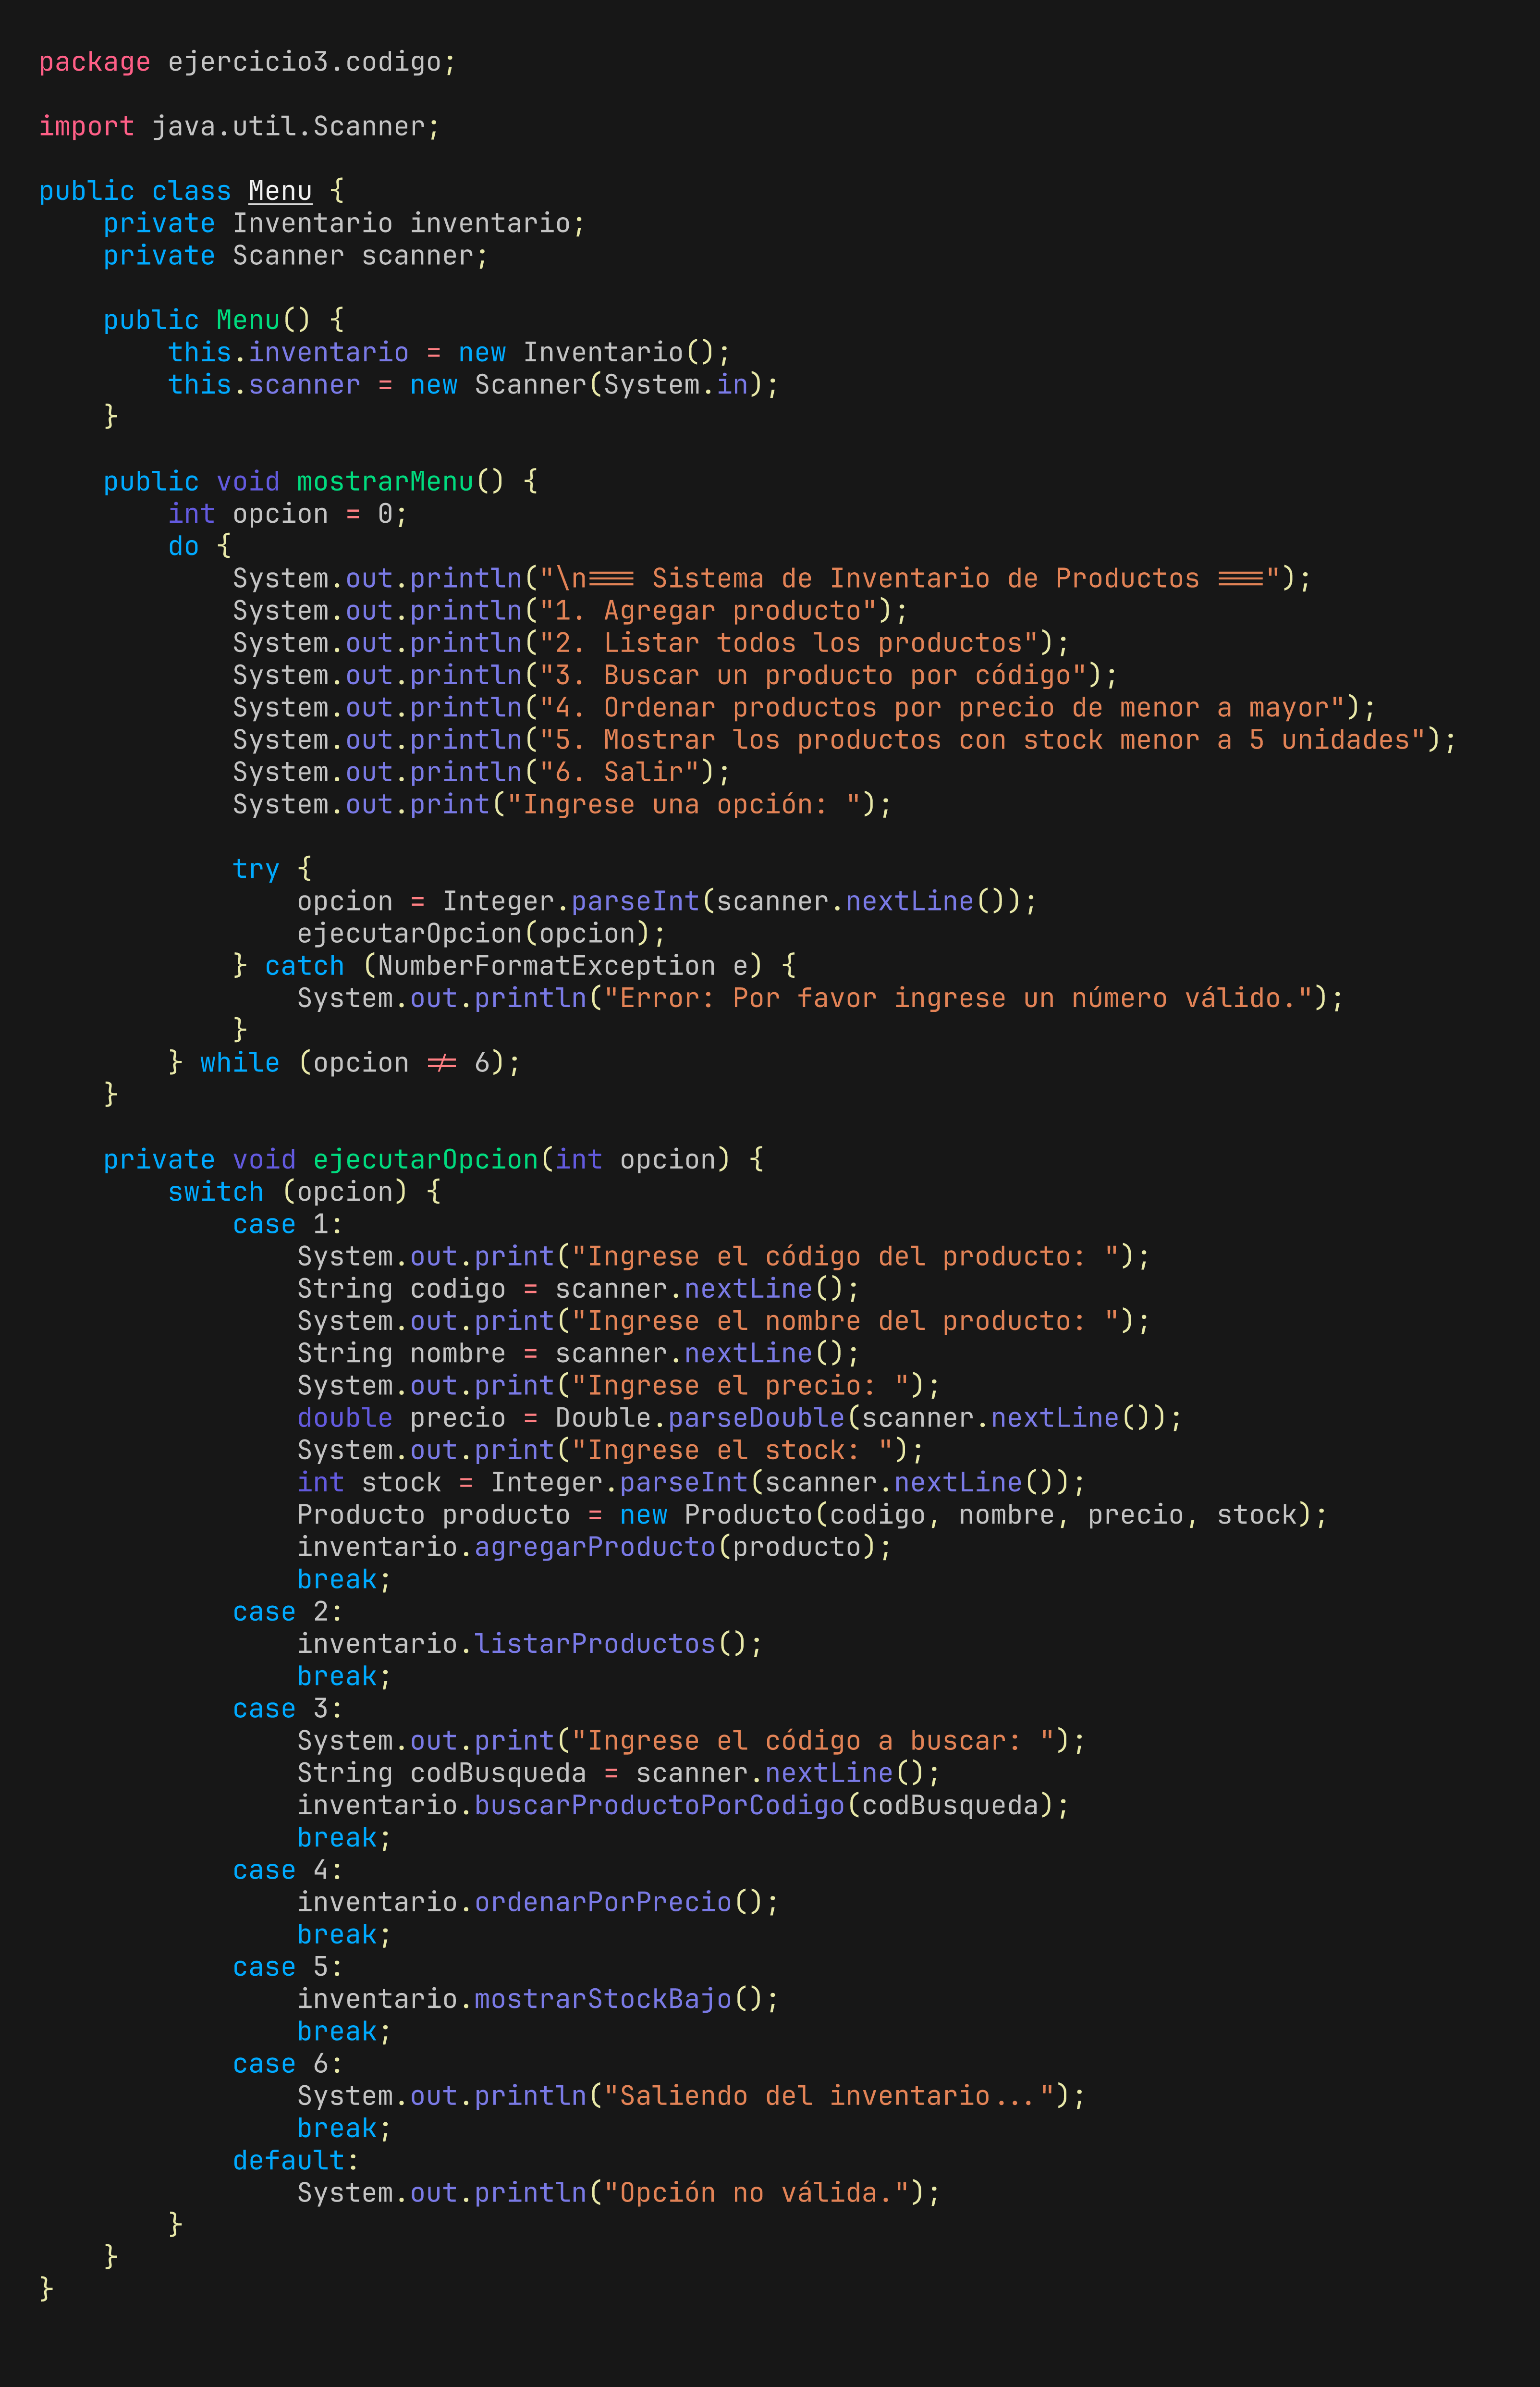
\includegraphics[width=0.8\textwidth]{ejercicio3/CAPTURAS_CODIGO/Menu.png}
    \caption{Código Fuente: Menu.png}
\end{figure}

\begin{figure}[H]
    \centering
    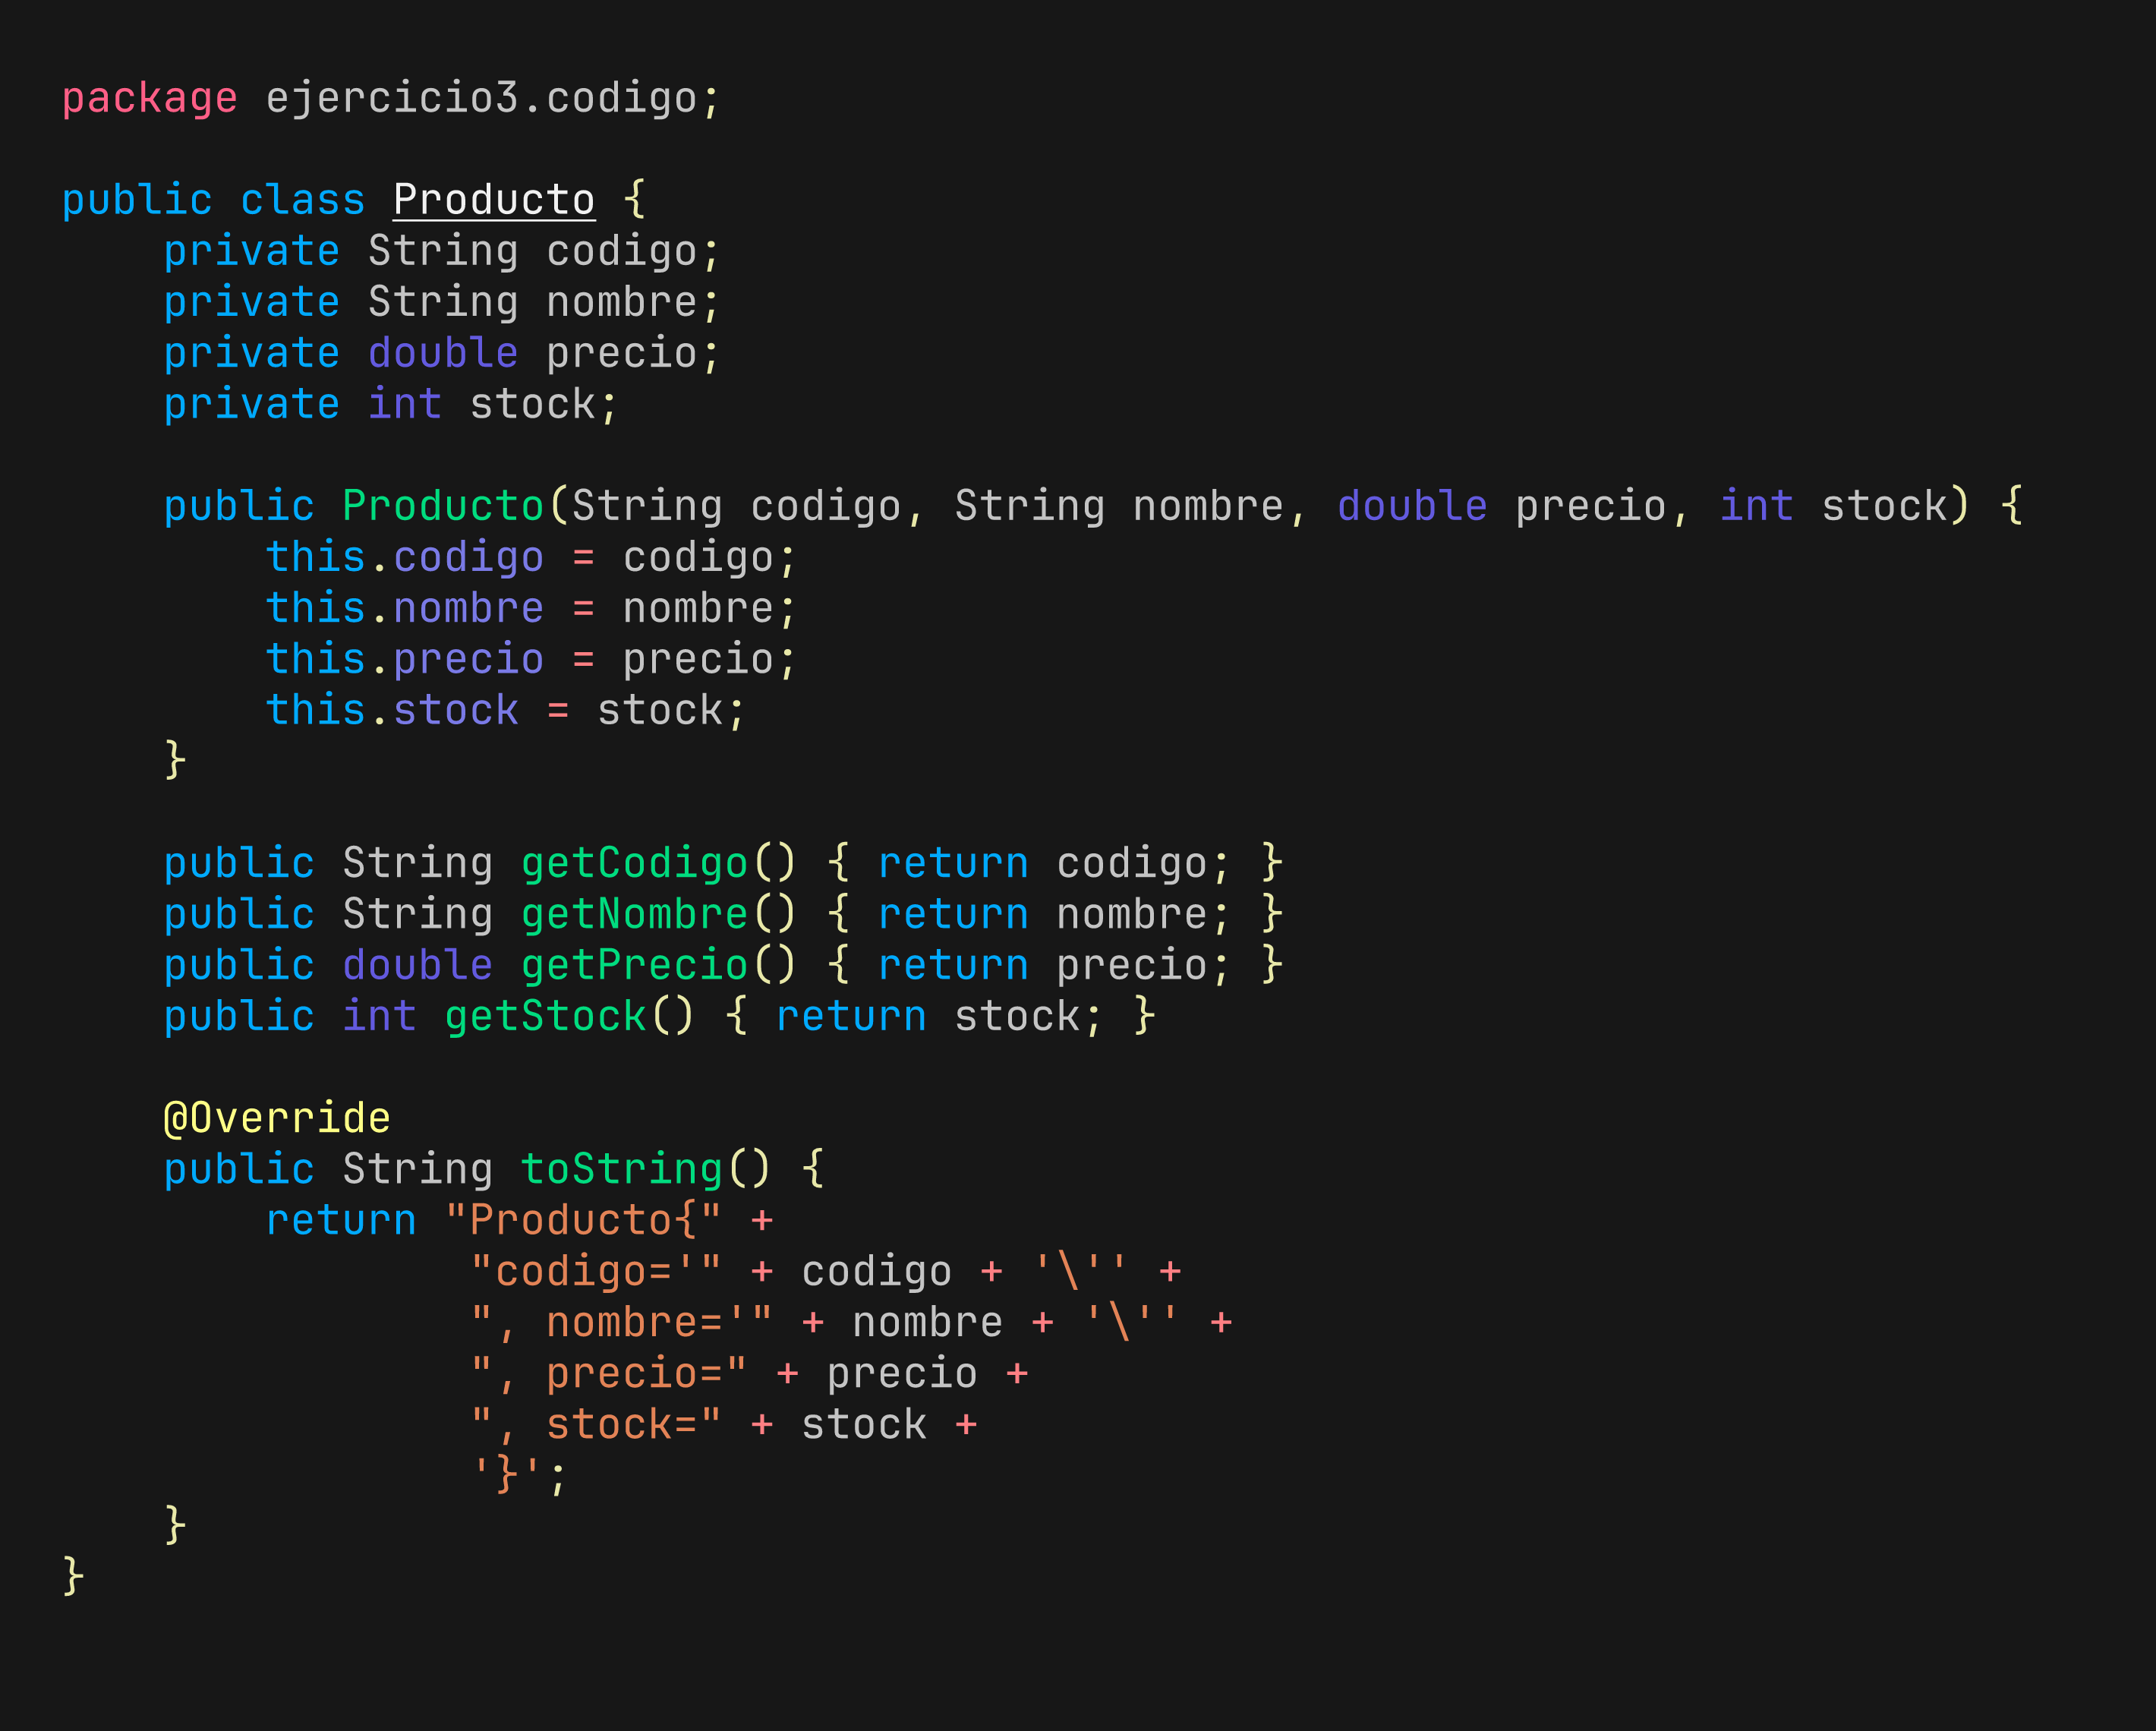
\includegraphics[width=0.8\textwidth]{ejercicio3/CAPTURAS_CODIGO/Producto.png}
    \caption{Código Fuente: Producto.png}
\end{figure}

\subsubsection*{Evidencias de Ejecución}
\begin{figure}[H]
    \centering
    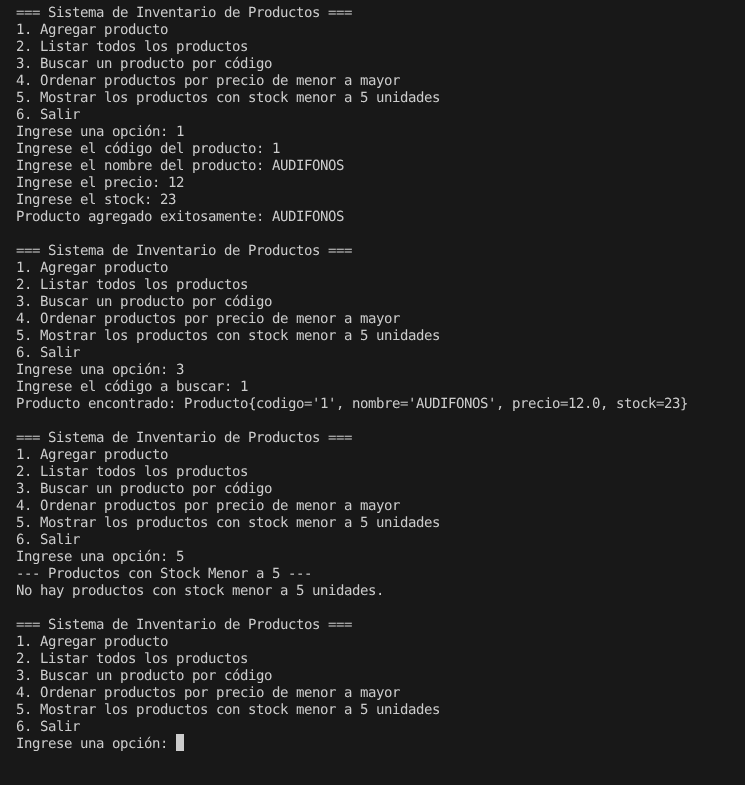
\includegraphics[width=0.8\textwidth]{ejercicio3/CAPTURAS_RESULTADO_CODIGO/image.png}
    \caption{Resultado de Ejecución - Reto 3}
\end{figure}

\subsection*{Reto 4}
Reto 4 - Caso de estudio: Control de tareas académicas

Desarrolle un programa para gestionar tareas académicas de estudiantes. Cada tarea tendrá código, descripción, prioridad y estado. El sistema debe permitir:
1. Registrar tareas en una lista
2. Buscar una tarea por código
3. Ordenar las tareas por prioridad
4. Marcar una tarea como completada
5. Guardar las tareas completadas en una pila
6. Mostrar la última tarea completada

\subsubsection*{Capturas de Pantalla del Código}
\begin{figure}[H]
    \centering
    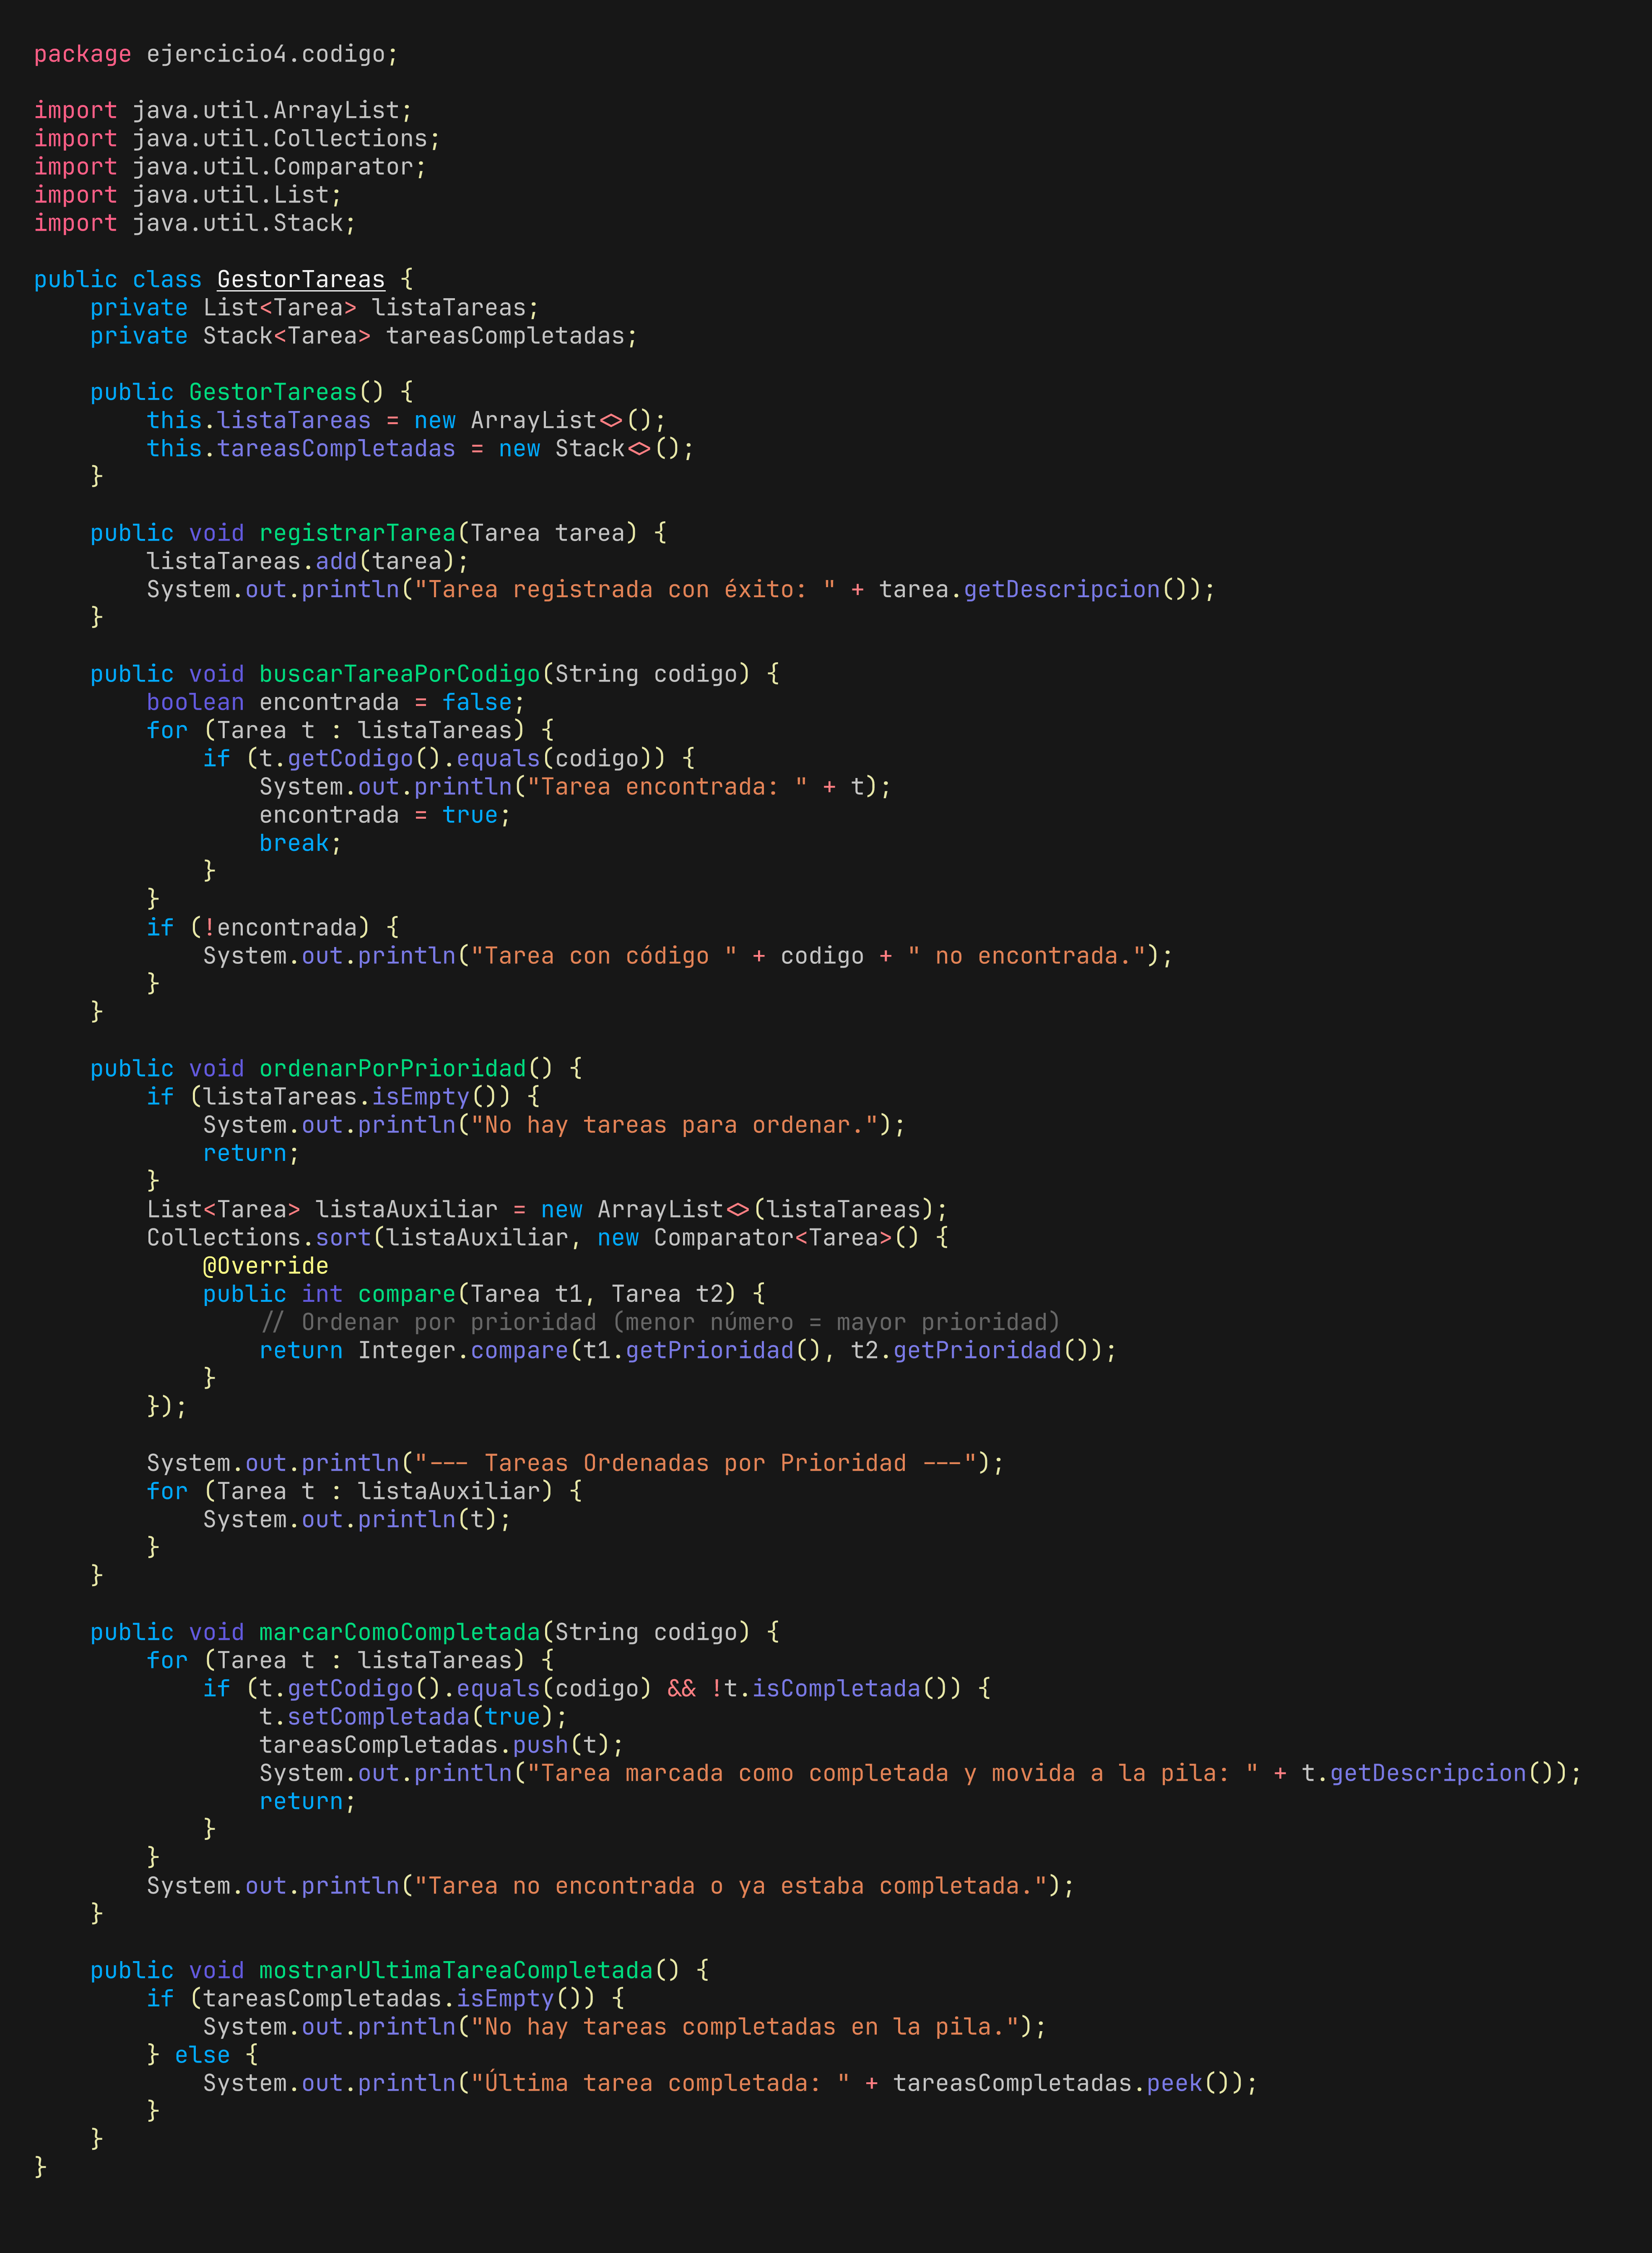
\includegraphics[width=0.8\textwidth]{ejercicio4/CAPTURAS_CODIGO/GestorTareas.png}
    \caption{Código Fuente: GestorTareas.png}
\end{figure}

\begin{figure}[H]
    \centering
    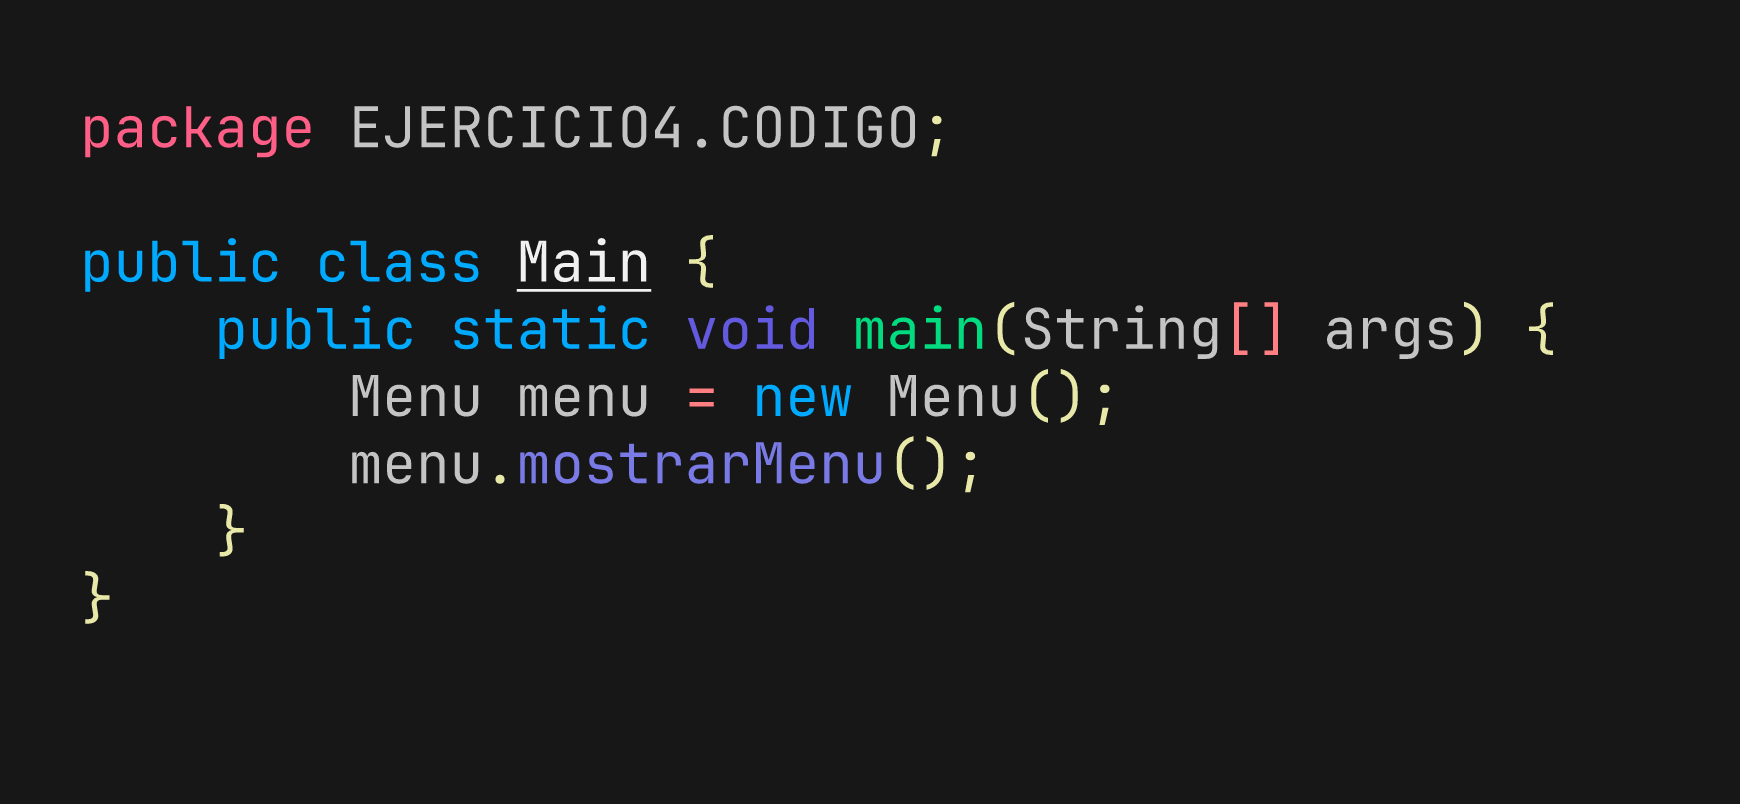
\includegraphics[width=0.8\textwidth]{ejercicio4/CAPTURAS_CODIGO/Main.png}
    \caption{Código Fuente: Main.png}
\end{figure}

\begin{figure}[H]
    \centering
    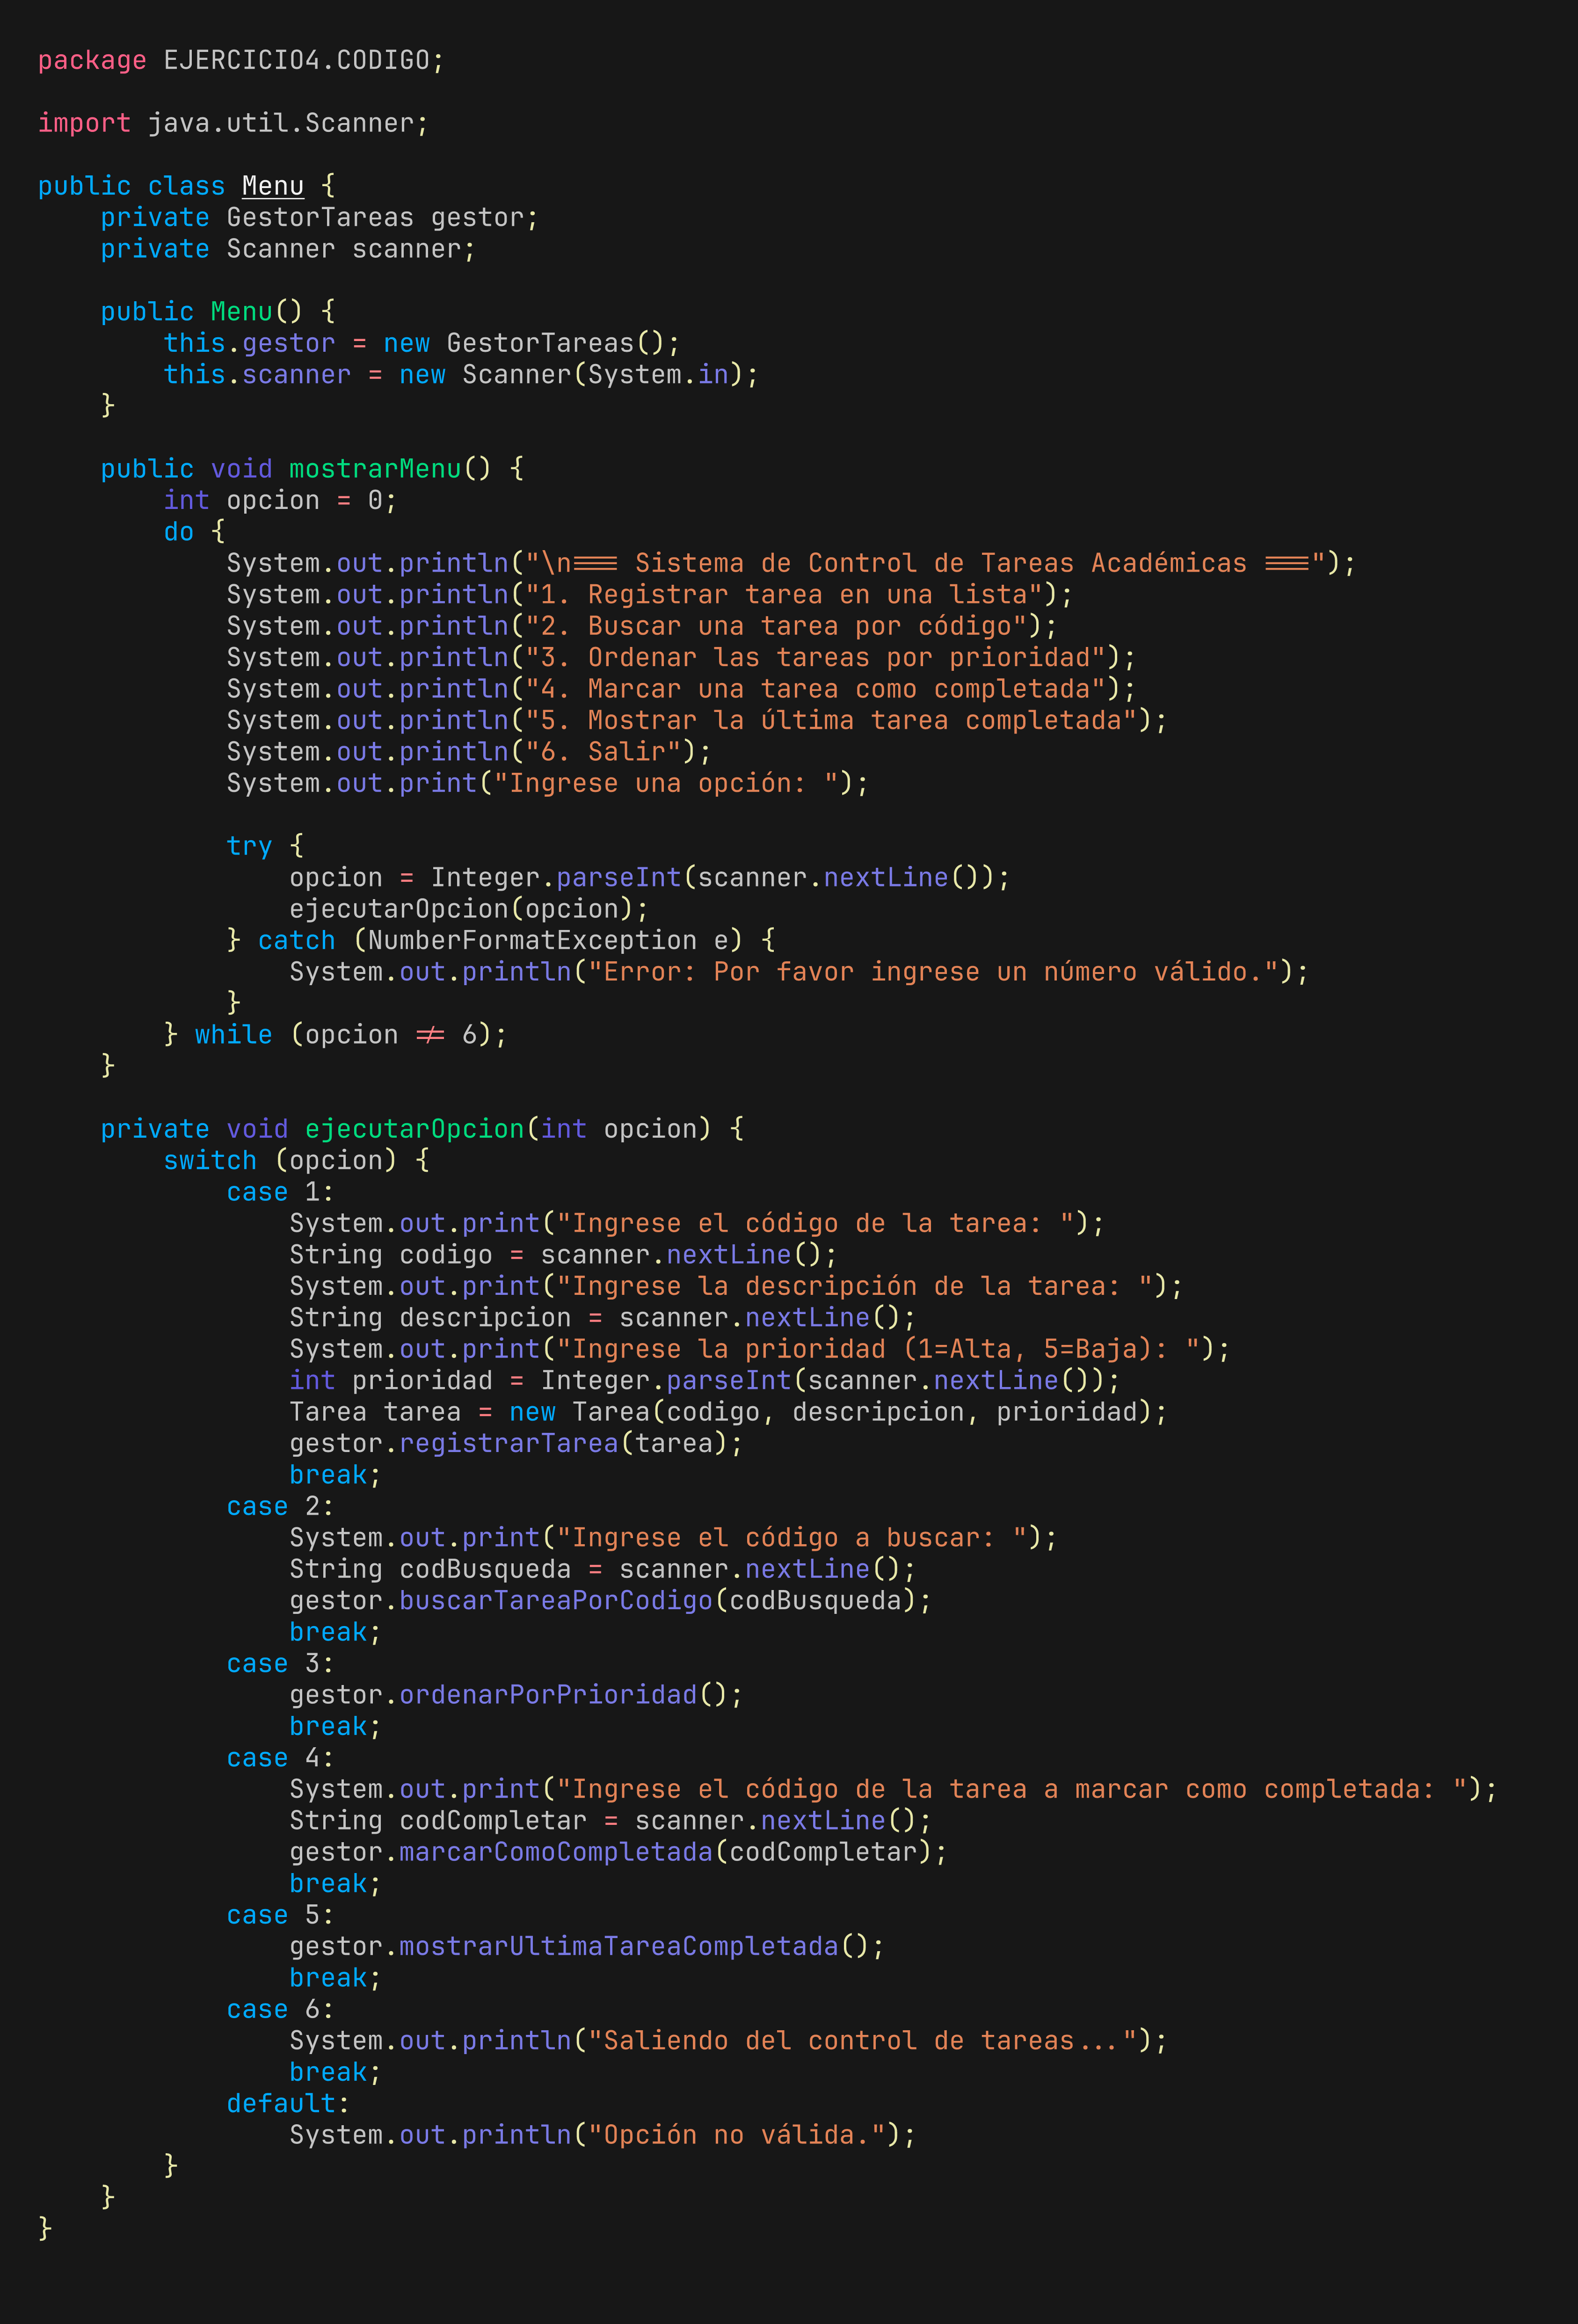
\includegraphics[width=0.8\textwidth]{ejercicio4/CAPTURAS_CODIGO/Menu.png}
    \caption{Código Fuente: Menu.png}
\end{figure}

\begin{figure}[H]
    \centering
    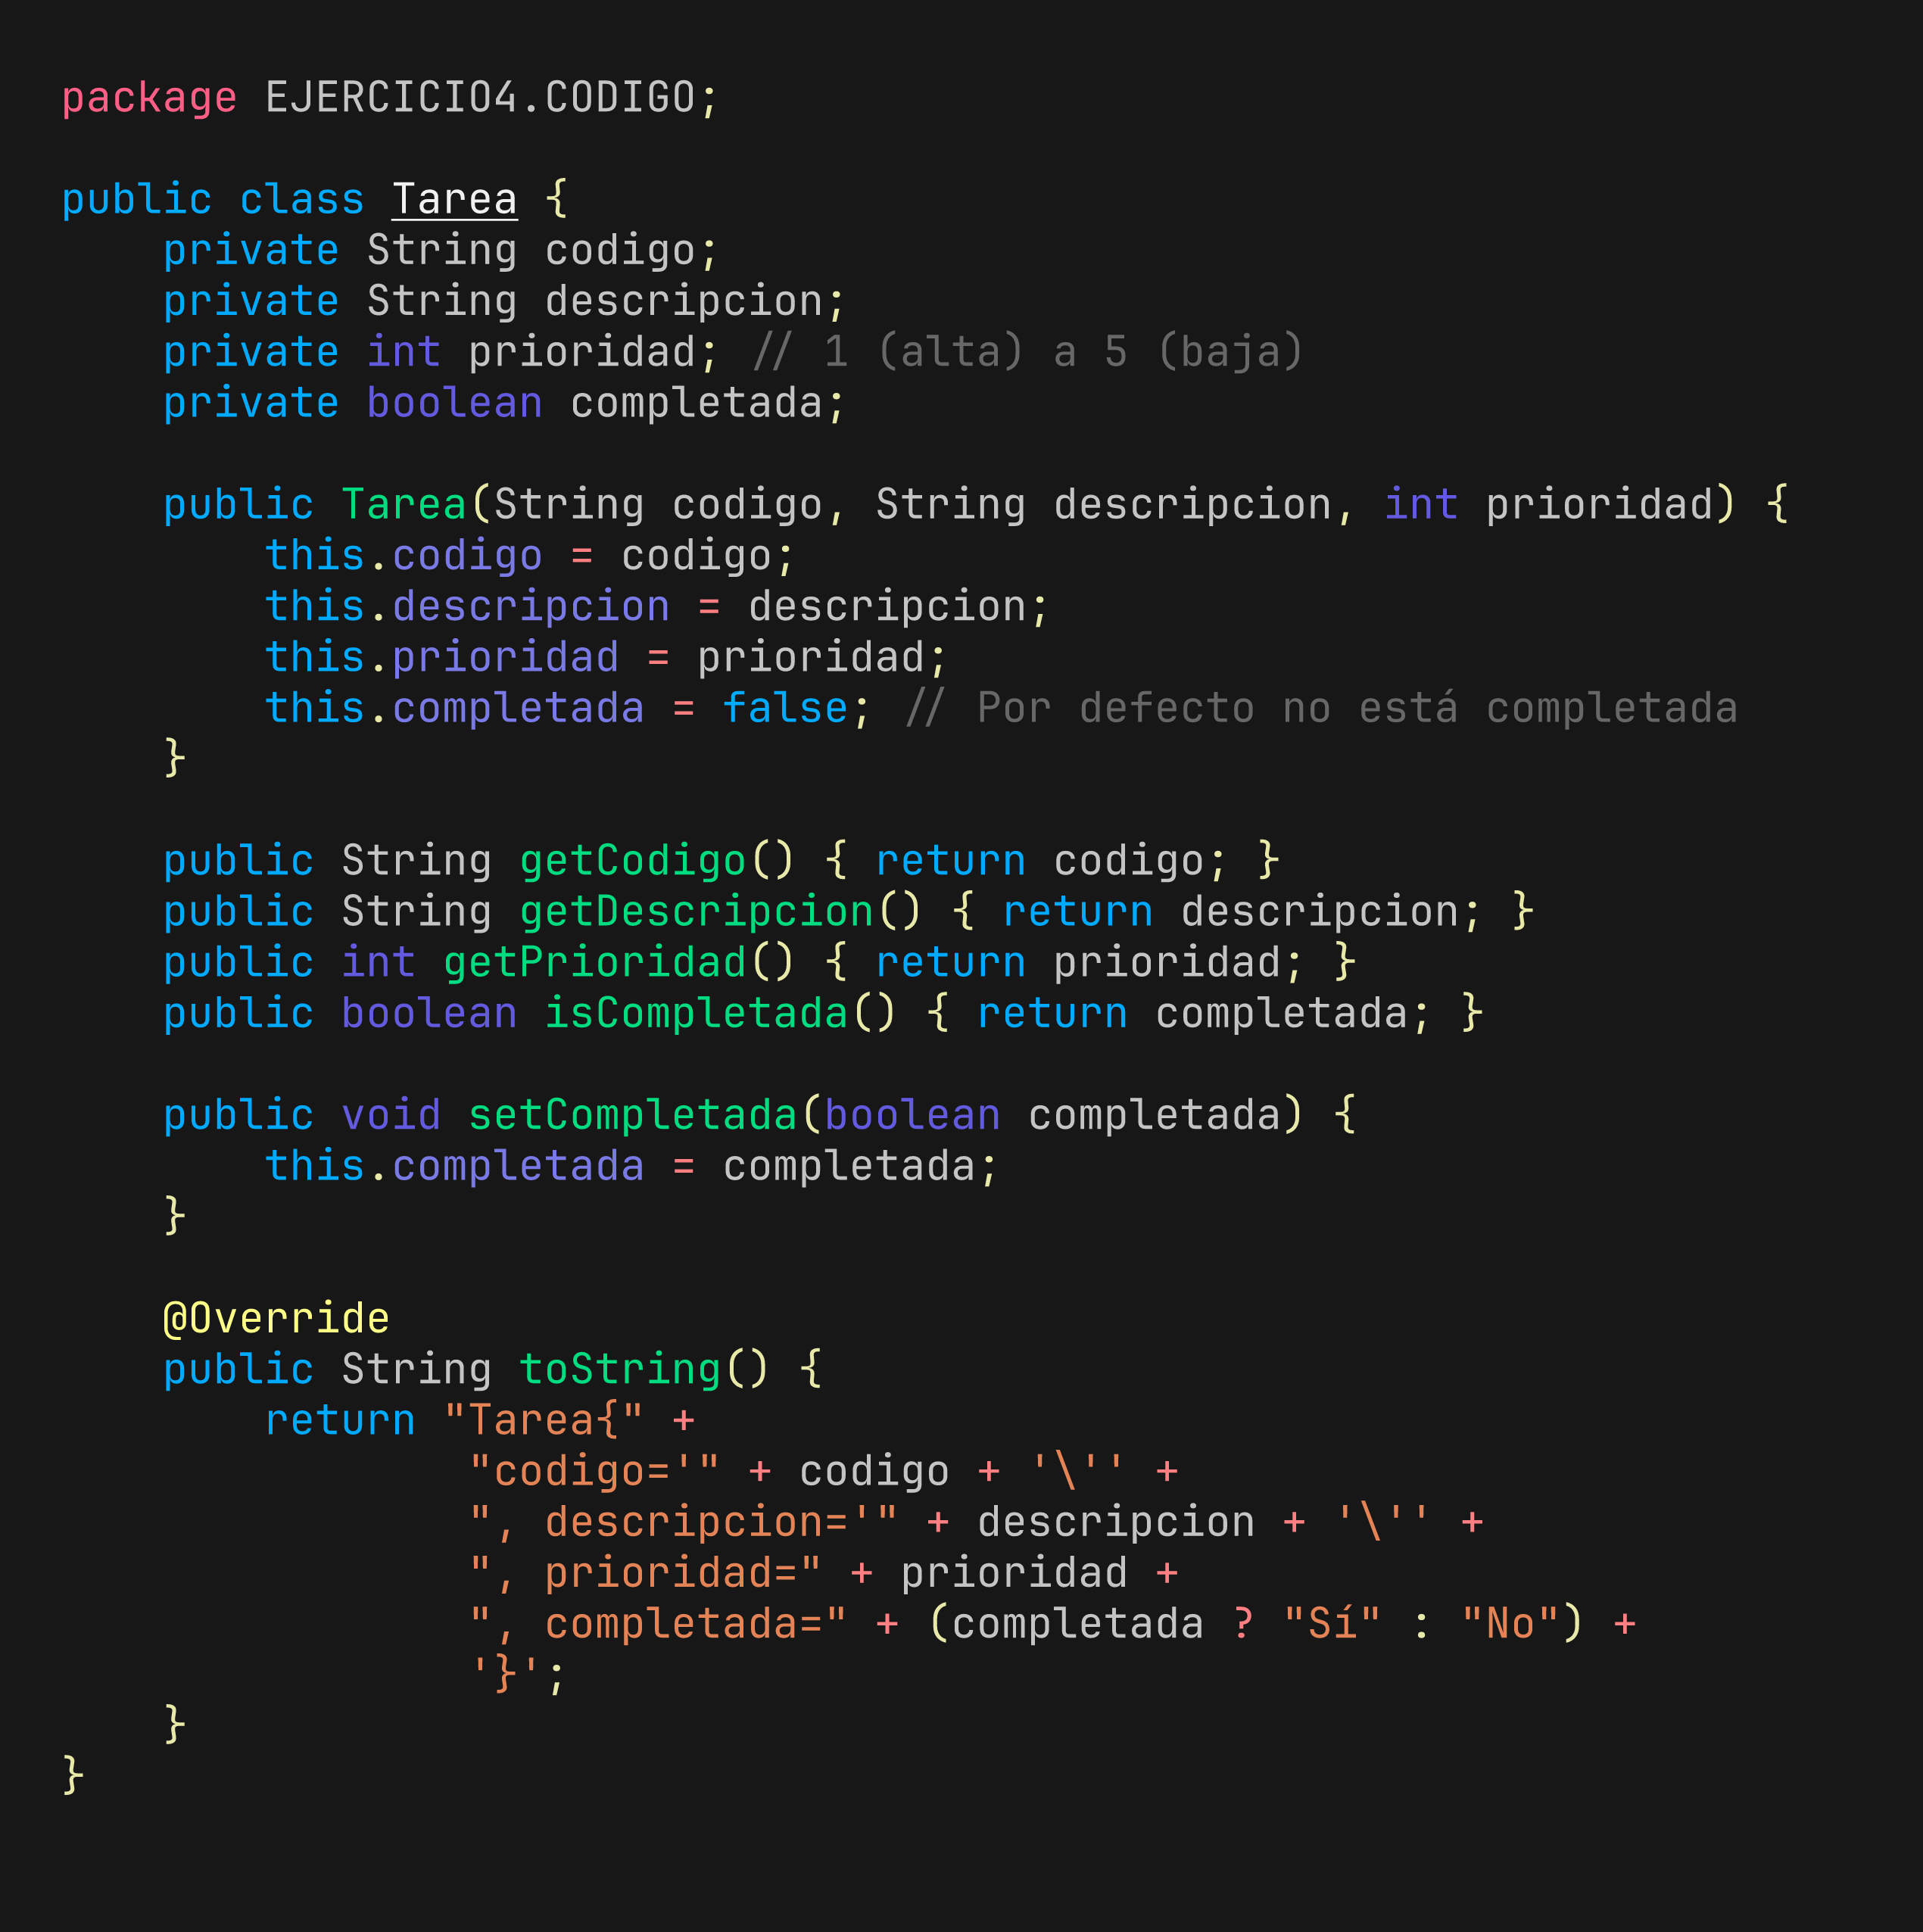
\includegraphics[width=0.8\textwidth]{ejercicio4/CAPTURAS_CODIGO/Tarea.png}
    \caption{Código Fuente: Tarea.png}
\end{figure}

\subsubsection*{Evidencias de Ejecución}
\begin{figure}[H]
    \centering
    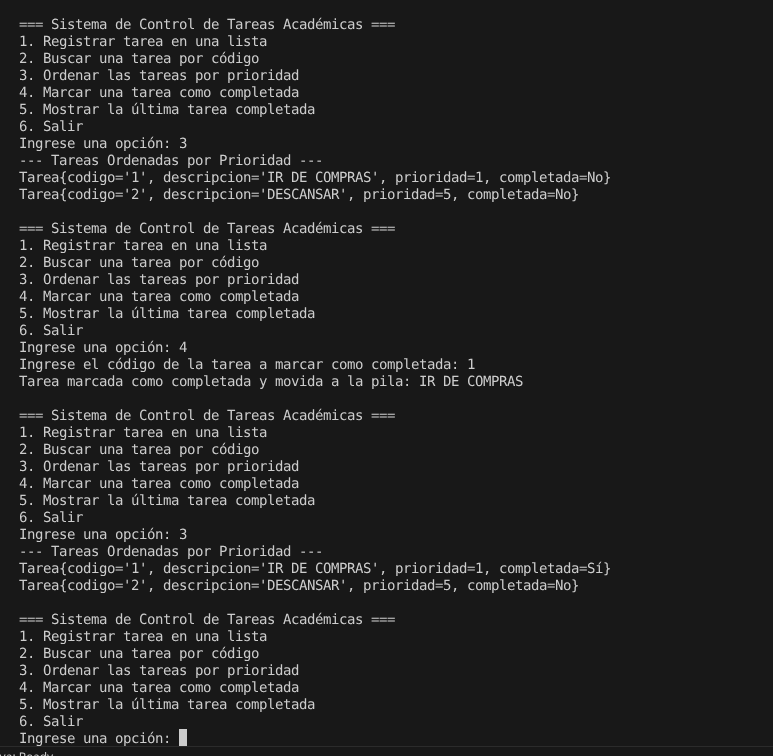
\includegraphics[width=0.8\textwidth]{ejercicio4/CAPTURAS_RESULTADO_CODIGO/image.png}
    \caption{Resultado de Ejecución - Reto 4}
\end{figure}

\section*{Enlaces de Entrega}
\begin{itemize}
    \item \textbf{Repositorio GitHub:} \url{https://github.com/Raul-Fernando-Cajiao-Garces/DEBER3}
    \item \textbf{Video Explicativo:} \url{https://drive.google.com/drive/folders/1-sCL-fiyJHtzv8PmKGGQZojoxlkY9-lI?usp=sharing}
\end{itemize}

\end{document}
